% audit.tex -- the reader's audit document.
%
% Build:  cd docs/audit && tectonic -X compile audit.tex   (or: tectonic audit.tex)
% Regenerate its inputs first:
%   python3 docs/audit/extract_lean.py
%   python3 docs/audit/gallery.py
%   python3 docs/audit/make_tables.py
%   python3 docs/audit/extract_lean.py --check     <- must exit 0
%
% Every line of Lean in this document is pulled from the source by
% extract_lean.py; every count is computed by gallery.py.  Nothing is retyped.

\documentclass[11pt]{article}

\usepackage[margin=0.9in]{geometry}
\usepackage{amsmath,amssymb}
\usepackage{booktabs}
\usepackage{graphicx}
\usepackage{microtype}
\usepackage{enumitem}
\usepackage{xcolor}
\usepackage[colorlinks=true,linkcolor=black,urlcolor=black,citecolor=black]{hyperref}
\usepackage{titlesec}
\usepackage{fancyvrb}

\titleformat{\section}{\large\bfseries}{\thesection.}{0.6em}{}
\titlespacing*{\section}{0pt}{16pt}{6pt}

\setlist[itemize]{leftmargin=1.2em,itemsep=2pt,topsep=3pt}
\setlist[enumerate]{leftmargin=1.5em,itemsep=2pt,topsep=3pt}

% lean_preamble.tex -- generated by docs/audit/extract_lean.py
% Macros used by lean_excerpts.tex.  Input this in the document preamble.
% The excerpts contain literal unicode for any glyph the extractor could not
% map; compile with XeLaTeX or LuaLaTeX, or extend UNICODE_MAP in the tool.
\providecommand{\leanline}[1]{\noindent\texttt{\small #1}\par}
\newenvironment{leandecl}[3]%
  {\par\medskip\noindent\textbf{\texttt{#1}}\hfill{\small\texttt{#2}:#3}\par
   \nopagebreak\smallskip\begingroup\setlength{\parindent}{0pt}}%
  {\endgroup\par\medskip}

% generated by docs/audit/make_tables.py -- do not edit by hand
\newcommand{\certcount}{38}
\newcommand{\galcount}{10}
\newcommand{\ndecls}{16}
\newcommand{\hllogpath}{\texttt{results/validation/2026-09-24\_headline\_build.log}}
\newcommand{\hllogdate}{2026-09-25T01:36:38Z}
\newcommand{\hljobs}{3{,}344}
\newcommand{\hllines}{83{,}020}
\newcommand{\hldepends}{408}
\newcommand{\hlsorry}{0}
\newcommand{\hlnative}{0}
\newcommand{\hlreplayed}{271}
\newcommand{\hlbuilt}{0}
\newcommand{\hlnaxioms}{3}
\newcommand{\hlparsed}{409}
\newcommand{\hlheadlines}{6 of 6}
\newcommand{\hlbadaxioms}{0}
\newcommand{\Lfourreq}{The requirement is that the build \emph{fail}. It does: that is case~L4 of the run recorded below.}
\newcommand{\Lfourupshot}{That is what shows the definitions are load-bearing and not decoration --- and it is what the run below shows. A reader who spends ten minutes on the 7 rows of \S2 is therefore checking text that genuinely determines the result, not prose sitting above proofs that would compile whatever it said.}
\newcommand{\locpP}{\texttt{lean/ResidualSymBase.lean}:23}
\newcommand{\locpQ}{\texttt{lean/ResidualSymBase.lean}:26}
\newcommand{\locSimpleClosed}{\texttt{lean/AKR9.lean}:71}
\newcommand{\locPair}{\texttt{lean/AKR9.lean}:81}
\newcommand{\locNoVertexOnOther}{\texttt{lean/AKR9.lean}:103}
\newcommand{\locsideP}{\texttt{lean/AKR9.lean}:109}
\newcommand{\locsideQ}{\texttt{lean/AKR9.lean}:112}
\newcommand{\locbdryP}{\texttt{lean/AKR9.lean}:115}
\newcommand{\locbdryQ}{\texttt{lean/AKR9.lean}:116}
\newcommand{\locpoints}{\texttt{lean/AKR9.lean}:119}
\newcommand{\locattainedCoincFree}{\texttt{lean/Pair9Shift.lean}:4314}
\newcommand{\locpointsleofcoincFree}{\texttt{lean/Pair9Shift.lean}:4223}
\newcommand{\locisGreatestofcoincFree}{\texttt{lean/Pair9Shift.lean}:4324}
\newcommand{\locnonVacuity}{\texttt{lean/Pair9Shift.lean}:5296}
\newcommand{\loccertPairnotle}{\texttt{lean/Pair9Shift.lean}:5252}
\newcommand{\locisGreatestattainedCoincFreeunique}{\texttt{lean/Pair9Shift.lean}:5272}


\newcommand{\code}[1]{\texttt{\small #1}}

\newsavebox{\trustboxbuf}
\newenvironment{trustbox}%
  {\par\medskip\setlength{\fboxsep}{9pt}%
   \begin{lrbox}{\trustboxbuf}%
   \begin{minipage}{\dimexpr\textwidth-2\fboxsep-2\fboxrule\relax}}%
  {\end{minipage}\end{lrbox}%
   \noindent\fcolorbox{black!35}{black!4}{\usebox{\trustboxbuf}}\par\medskip}

\title{\bfseries Two simple heptagons sharing no vertex meet in at most 38 points:\\
what the machine checked, and what it did not}
\author{An audit document for the Lean development,\\ written for readers with or without Lean experience}
\date{Revised 4 October 2026 (first version 24 September 2026)}

\setcounter{section}{-1}
\begin{document}
\maketitle
\thispagestyle{empty}

\vspace{-1.2\baselineskip}

\begin{trustbox}
\textbf{In one paragraph.} A Lean~4 development in this repository contains a
kernel-checked theorem: \emph{if two simple heptagons in the plane share no
vertex and their boundaries meet in finitely many points, then the boundaries
meet in at most $38$ points; and $38$ is attained.} This includes every pair in
general position. The recorded build of the theorem shows no \code{sorry}, no
axiom declared by this project, and no \code{native\_decide}. The theorem is
\textbf{not} by itself the statement $f(7,7)=38$, which ranges also over pairs
that share vertices: that step uses the vertex-coincidence reduction of \S9.1
of Ackerman--Keszegh--Rote, which is not formalized here and whose
applicability to these exact definitions this project has not fully checked
(\S\ref{sec:notproved}). This document sets out the formal statement, the
evidence for it, and the limits of that evidence.
\end{trustbox}

\section{What the evidence does and does not establish}

\paragraph{Kernel checking.} A Lean file is a set of instructions for
constructing proof objects, which Lean's kernel checks against a fixed set of
inference rules. If the development builds, the kernel has accepted a proof of
each theorem's formal statement, under its stated hypotheses and Lean's
foundational axioms, relative to the correctness of Lean itself and of the
Mathlib definitions the statements use. This development is 1{,}779
\code{.lean} files and about 1.6 million lines; most files are generated case
enumerations, and the proofs of the headline theorems are long generated
propagation chains. They are not written to be read line by line, and reading
them is not the usual way such a development is reviewed. Kernel checking does
not establish that a formal statement says what its author intends, and it
does not discharge the statement's hypotheses.

\paragraph{The statement and definitions.} What a reviewer must read is the
statement and the definitions it uses. If \code{points9} denoted the wrong
set, or \code{SimpleClosed} encoded more than simplicity, a correct
kernel-checked proof would establish something other than the intended
result. The statement surface quoted here is \ndecls\ declarations, and the
seven that carry the content are printed in \S2 beside a reading in ordinary
mathematics. Other risks remain alongside the definitions: a hypothesis
stronger than intended (addressed for satisfiability by \S\ref{sec:nonvac}), a mismatch
between the code quoted here and the code that was built (addressed partly by
the drift check of \S2), and the external reduction (\S\ref{sec:notproved}).

\paragraph{The axiom check.}
Lean's \code{\#print axioms} lists the axioms a declaration's proof depends on,
transitively. Three kinds of dependency are relevant here, and the
repository's axiom checker looks for each:

\begin{itemize}
\item \code{sorry}, a placeholder for a missing proof. A file containing it
  still compiles, with a warning, and the build exits~0. It appears in the
  axiom list as \code{sorryAx}.
\item A declared \code{axiom}, a statement asserted without proof. It appears
  by name.
\item \code{native\_decide}, which evaluates a goal with compiled code rather
  than in the kernel, enlarging the trusted code base to the compiler. It
  appears as \code{Lean.ofReduceBool}.
\end{itemize}

The expected output for the headline theorems is
\[
  \texttt{[propext, Classical.choice, Quot.sound]},
\]
Lean's standard foundational axioms, which Mathlib also uses. The check is
evidence about the declarations whose axiom lists are printed and parsed. It
does not show that a statement has the intended meaning, it does not discharge
hypotheses, and it does not detect errors in Lean itself.

\paragraph{Recorded builds.} The repository's GitHub Actions workflow builds
the headline target from a fresh checkout on a GitHub-hosted runner, runs the
axiom check, and runs the group-A tests of \S4. Two runs have passed
(\S\ref{sec:ci}). A run records that the committed workflow passed at one
revision. The repository owner writes the workflow, so the run shows what that
workflow checked, not an independent party's choice of checks. It is not a
mathematical review.

\paragraph{What a reader still has to judge.}
\begin{enumerate}
\item \textbf{The toolchain:} that Lean's kernel, and the Mathlib definitions
  used in the statement, are correct. This is assumed by every Lean
  formalization.
\item \textbf{The statement:} that the formal statement in \S2 expresses the
  intended theorem. The table in \S2 supports this check; it is easier for a
  reader who knows Lean.
\item \textbf{The connection between this document and the code:} that what
  is quoted here is what was built (\S\S2 and~5).
\item \textbf{The external reduction:} AKR \S9.1, and whether it applies to
  these definitions (\S\ref{sec:notproved}).
\end{enumerate}

\section{The claim, in ordinary mathematics}

\begin{trustbox}
\textbf{Proved.} Let $P$ and $Q$ be simple closed heptagons in the plane ---
seven vertices each, sides $[P_i,P_{i+1}]$ and $[Q_j,Q_{j+1}]$ for
$i,j\in\mathbb{Z}/7$, each polygon a closed curve that does not cross itself.
Suppose $\partial P\cap\partial Q$ is finite and no vertex of $P$ is equal to
a vertex of $Q$. Then $\#(\partial P\cap\partial Q)\le 38$, and there is such a
pair for which the count is exactly $38$; so $38$ is the maximum over such
pairs. Every pair in general position satisfies these hypotheses.

\medskip
\textbf{Hypotheses, not conclusions.} Finiteness and ``no shared vertex'' are
hypotheses of the theorem, written out explicitly. That every pair of simple
heptagons with finite intersection can be replaced by one with no shared
vertex, again simple and with no fewer intersection points, is a separate
\emph{reduction}: it is the subject of \S9.1 of Ackerman, Keszegh and Rote,
and it is not formalized here (\S\ref{sec:notproved}).
\end{trustbox}

\noindent Two remarks on what is \emph{not} assumed, because these are the
places where a formal statement is most easily narrower than intended.

\emph{No general position.} Three collinear vertices are allowed. A straight
vertex --- where two consecutive sides are collinear --- is allowed. A vertex of
one polygon lying in the \emph{interior} of a side of the other is allowed, and
is the case AKR \S9.2 removes by a perturbation argument; here it is proved,
not assumed away. The only degeneracy excluded is vertex-equals-vertex.

\emph{Points, not crossings.} The quantity bounded is the cardinality of a set
of points of the plane. A tangential touch that does not cross counts as one
point; a point where three sides concur counts once, not twice. This is the
harder thing to bound and the thing the question actually asks.

\section{The statement, beside the mathematics}

This is the part to read. The left column is the claim in ordinary
mathematical English; the right column is the Lean source, quoted verbatim by
\code{docs/audit/extract\_lean.py} from the files and line numbers shown.
\textbf{Your task is to decide whether the two columns say the same thing.}
Nothing else in this document depends on your knowing any Lean: the notation
you need is $\forall$, $\wedge$ (and), $\to$ (implies), $\cup$, $\cap$,
\code{Fin 7} $=\mathbb{Z}/7$ with wraparound on \code{+}, and
\code{segment $\mathbb{R}$ a b} $=[a,b]$, the closed segment.

% generated by docs/audit/make_tables.py -- do not edit by hand
\begingroup
\setlength{\tabcolsep}{4pt}
\renewcommand{\arraystretch}{1.15}
\noindent\begin{tabular}{@{}p{0.27\textwidth}@{\hspace{9pt}}p{0.70\textwidth}@{}}
\toprule
\textbf{the mathematics} & \textbf{the Lean, verbatim}\\
\bottomrule
\end{tabular}\par\smallskip
\noindent\begin{tabular}{@{}p{0.27\textwidth}@{\hspace{9pt}}p{0.70\textwidth}@{}}
\textbf{(1)}\ $P$ is a closed heptagon that does not cross itself: no side is a point, non-adjacent sides are disjoint, and two consecutive sides meet exactly in the vertex they share. & {\scriptsize\ttfamily\setlength{\parindent}{0pt}\raggedright
\mbox{}def~SimpleClosed~(W~:~Fin~7~$\to$~$\mathbb{R}$~$\times$~$\mathbb{R}$)~:~Prop~:=\\[-1pt]
\mbox{}~~($\forall$~i~:~Fin~7,~W~i~$\ne$~W~(i~+~1))~$\land$\\[-1pt]
\mbox{}~~($\forall$~i~j~:~Fin~7,~$\lnot$~LowerBound.Adjacent~i~j~$\to$\\[-1pt]
\mbox{}~~~~~~Disjoint~(segment~$\mathbb{R}$~(W~i)~(W~(i~+~1)))~(segment~$\mathbb{R}$~(W~j)~(W~(j~+~1))))~$\land$\\[-1pt]
\mbox{}~~($\forall$~i~:~Fin~7,\\[-1pt]
\mbox{}~~~~~~segment~$\mathbb{R}$~(W~i)~(W~(i~+~1))~$\cap$~segment~$\mathbb{R}$~(W~(i~+~1))~(W~(i~+~2))\\[-1pt]
\mbox{}~~~~~~~~=~\{W~(i~+~1)\})\\[-1pt]
}\par\smallskip{\footnotesize\ttfamily lean/AKR9.lean:71}\\
\end{tabular}
\par\smallskip\noindent\hspace*{0.29\textwidth}\begin{minipage}{0.70\textwidth}{\footnotesize\textit{Note.}\ This is simplicity \emph{as a curve} and nothing more. Three collinear vertices are deliberately allowed --- a straight vertex is not excluded here. \texttt{Adjacent} is cyclic adjacency on $\mathbb{Z}/7$.}\end{minipage}
\par\medskip\noindent\rule{\textwidth}{0.3pt}\par\smallskip
\noindent\begin{tabular}{@{}p{0.27\textwidth}@{\hspace{9pt}}p{0.70\textwidth}@{}}
\textbf{(2)}\ The object under study is an ordered pair $(P,Q)$ of such heptagons in the plane. Nothing else is assumed about it. & {\scriptsize\ttfamily\setlength{\parindent}{0pt}\raggedright
\mbox{}structure~Pair9~where\\[-1pt]
\mbox{}~~/--~The~fourteen~vertices:~`P`~is~`0..6`,~`Q`~is~`7..13`.~-/\\[-1pt]
\mbox{}~~V~:~Fin~14~$\to$~$\mathbb{R}$~$\times$~$\mathbb{R}$\\[-1pt]
\mbox{}~~simpleP~:~SimpleClosed~(fun~i~:~Fin~7~=>~V~(pP~i))\\[-1pt]
\mbox{}~~simpleQ~:~SimpleClosed~(fun~i~:~Fin~7~=>~V~(pQ~i))\\[-1pt]
}\par\smallskip{\footnotesize\ttfamily lean/AKR9.lean:81}\\
\end{tabular}
\par\smallskip\noindent\hspace*{0.29\textwidth}\begin{minipage}{0.70\textwidth}{\footnotesize\textit{Note.}\ The fourteen vertices are one function \texttt{V}; \texttt{pP\,i} $=i$ and \texttt{pQ\,i} $=7+i$ split them. There is no general-position field, and no non-degeneracy field. The two \texttt{simple} fields are the whole hypothesis.}\end{minipage}
\par\medskip\noindent\rule{\textwidth}{0.3pt}\par\smallskip
\noindent\begin{tabular}{@{}p{0.27\textwidth}@{\hspace{9pt}}p{0.70\textwidth}@{}}
\textbf{(3)}\ $\partial P=\bigcup_{i\in\mathbb{Z}/7}[P_i,P_{i+1}]$, the union of the seven closed sides; likewise $\partial Q$. & {\scriptsize\ttfamily\setlength{\parindent}{0pt}\raggedright
\mbox{}def~bdryP9~(R~:~Pair9)~:~Set~($\mathbb{R}$~$\times$~$\mathbb{R}$)~:=~$\bigcup$~i~:~Fin~7,~sideP9~R~i\\[-1pt]
}\par\smallskip{\footnotesize\ttfamily lean/AKR9.lean:115}\\
\end{tabular}
\par\smallskip\noindent\hspace*{0.29\textwidth}\begin{minipage}{0.70\textwidth}{\footnotesize\textit{Note.}\ \texttt{segment $\mathbb{R}$ a b} is Mathlib's \emph{closed} segment $\{(1-t)a+tb : 0\le t\le 1\}$, so endpoints are included. \texttt{sideP9} is that segment; \texttt{bdryQ9} is the same with \texttt{pQ}.}\end{minipage}
\par\medskip\noindent\rule{\textwidth}{0.3pt}\par\smallskip
\noindent\begin{tabular}{@{}p{0.27\textwidth}@{\hspace{9pt}}p{0.70\textwidth}@{}}
\textbf{(4)}\ The set being counted is $\partial P\cap\partial Q$: the points of the plane lying on both boundaries. & {\scriptsize\ttfamily\setlength{\parindent}{0pt}\raggedright
\mbox{}def~points9~(R~:~Pair9)~:~Set~($\mathbb{R}$~$\times$~$\mathbb{R}$)~:=~bdryP9~R~$\cap$~bdryQ9~R\\[-1pt]
}\par\smallskip{\footnotesize\ttfamily lean/AKR9.lean:119}\\
\end{tabular}
\par\smallskip\noindent\hspace*{0.29\textwidth}\begin{minipage}{0.70\textwidth}{\footnotesize\textit{Note.}\ A set of points, not a list of crossings and not a multiset. A point where three sides concur is one element, not two.}\end{minipage}
\par\medskip\noindent\rule{\textwidth}{0.3pt}\par\smallskip
\noindent\begin{tabular}{@{}p{0.27\textwidth}@{\hspace{9pt}}p{0.70\textwidth}@{}}
\textbf{(5)}\ \emph{Assumed:} no vertex of $P$ equals a vertex of $Q$. (This is the conclusion of AKR \S9.1; see \S7.) & {\scriptsize\ttfamily\setlength{\parindent}{0pt}\raggedright
\mbox{}def~attainedCoincFree~:~Set~$\mathbb{N}$~:=\\[-1pt]
\mbox{}~~\{~n~|~$\exists$~R~:~Pair9,~(points9~R).Finite~$\land$\\[-1pt]
\mbox{}~~~~~~($\forall$~v~j~:~Fin~7,~R.V~(pP~v)~$\ne$~R.V~(pQ~j))~$\land$~(points9~R).ncard~=~n~\}\\[-1pt]
}\par\smallskip{\footnotesize\ttfamily lean/Pair9Shift.lean:4314}\\
\end{tabular}
\par\smallskip\noindent\hspace*{0.29\textwidth}\begin{minipage}{0.70\textwidth}{\footnotesize\textit{Note.}\ The middle clause is the assumption, written out. It forbids \emph{equality} of vertices only --- a vertex lying in the interior of the other polygon's side is \emph{not} excluded, and is handled by the proof.}\end{minipage}
\par\medskip\noindent\rule{\textwidth}{0.3pt}\par\smallskip
\noindent\begin{tabular}{@{}p{0.27\textwidth}@{\hspace{9pt}}p{0.70\textwidth}@{}}
\textbf{(6)}\ If $\partial P\cap\partial Q$ is finite and $P,Q$ share no vertex, then $\#(\partial P\cap\partial Q)\le 38$. & {\scriptsize\ttfamily\setlength{\parindent}{0pt}\raggedright
\mbox{}theorem~points9\_le\_38\_of\_coincFree~(R~:~Pair9)~(hfin~:~(points9~R).Finite)\\[-1pt]
\mbox{}~~~~(hcoinc~:~$\forall$~v~j~:~Fin~7,~R.V~(pP~v)~$\ne$~R.V~(pQ~j))~:\\[-1pt]
\mbox{}~~~~(points9~R).ncard~$\le$~38~:=~by\\[-1pt]
\mbox{}~~obtain~$\langle$Rend,~hD,~hE,~hb$\rangle$~:=~exists\_chain\_deg\_free~\_~R~hfin~hcoinc~rfl\\[-1pt]
\mbox{}~~exact~points9\_le\_38\_of\_joint~R~Rend~hfin~hb~hD~hE\\[-1pt]
}\par\smallskip{\footnotesize\ttfamily lean/Pair9Shift.lean:4223}\\
\end{tabular}
\par\smallskip\noindent\hspace*{0.29\textwidth}\begin{minipage}{0.70\textwidth}{\footnotesize\textit{Note.}\ \texttt{ncard} is the cardinality of a set as a natural number. \texttt{hfin} is the finiteness hypothesis; without it the count is not a number at all (see the last row of \S3).}\end{minipage}
\par\medskip\noindent\rule{\textwidth}{0.3pt}\par\smallskip
\noindent\begin{tabular}{@{}p{0.27\textwidth}@{\hspace{9pt}}p{0.70\textwidth}@{}}
\textbf{(7)}\ $38$ is attained, and is the largest attained value: it is the maximum, not merely an upper bound. & {\scriptsize\ttfamily\setlength{\parindent}{0pt}\raggedright
\mbox{}theorem~isGreatest\_38\_of\_coincFree~:~IsGreatest~attainedCoincFree~38~:=~by\\[-1pt]
\mbox{}~~refine~$\langle$$\langle$AKR9.certPair9,~certPair9\_finite,~certPair9\_coincFree,\\[-1pt]
\mbox{}~~~~AKR9.certPair9\_ncard$\rangle$,~?\_$\rangle$\\[-1pt]
\mbox{}~~rintro~n~$\langle$R,~hfin,~hco,~rfl$\rangle$\\[-1pt]
\mbox{}~~exact~points9\_le\_38\_of\_coincFree~R~hfin~hco\\[-1pt]
}\par\smallskip{\footnotesize\ttfamily lean/Pair9Shift.lean:4324}\\
\end{tabular}
\par\smallskip\noindent\hspace*{0.29\textwidth}\begin{minipage}{0.70\textwidth}{\footnotesize\textit{Note.}\ \texttt{IsGreatest S a} unfolds to $a\in S \wedge \forall b\in S,\ b\le a$. The membership half is the explicit certificate of \S3; the bound half is the row above.}\end{minipage}
\par\medskip\noindent\rule{\textwidth}{0.3pt}\par\smallskip
\endgroup


\paragraph{The drift check.} \code{extract\_lean.py --check} recomputes the
SHA-256 of each of the \ndecls\ quoted declarations and compares it against the
lockfile written when this document was generated. If one of them has been
renamed, removed, or altered by one character, it exits~1 and names it. It is
part of the documented procedure for building this PDF. It covers only the
quoted text: a change to a definition those declarations use but that is not
quoted here --- for example \code{LowerBound.Adjacent}, or Mathlib's
\code{segment} --- would not be detected by it.

\paragraph{One thing this table is not.} The repository contains a
\emph{second} chain that also ends at the number $38$ ---
\code{Heptagon.MainTheorem.isGreatest\_38}, over integer-coordinate
combinatorial configurations --- and \S5 prints its axiom line alongside these.
It is not the theorem above: it carries three explicit hypotheses that that
route does not itself prove, and \S5 sets them out. The six axiom lines in
\S5 are six statements with different hypotheses, not six versions of one
result. The claim this document makes is the one in the table above, and nothing in \S\S1--4 or~\ref{sec:nonvac} depends on the other chain.

\section{The gallery: hand-countable pictures beside the computed count}

The definitions in \S2 are set-theoretic. This section checks that they compute
what you would count by eye. \code{docs/audit/gallery.py} transcribes the same
predicates into Python --- \code{orientR}, \code{SimpleClosed},
\code{Adjacent}, \code{points9}, each annotated with the Lean file and line it
came from --- draws \galcount\ configurations, and circles and numbers every
point of $\partial P\cap\partial Q$. All arithmetic is exact rational
arithmetic (\code{fractions.Fraction}); no floating point is used for any
geometric decision. The tool self-tests 33 properties on startup and aborts if
any fails, including a sweep confirming its segment-intersection routine agrees
with the textbook orientation test on all 6{,}561 segment pairs over a
$3\times3$ grid.

\medskip
\noindent\textbf{Lead with the certificate.} Figure~1 is
\code{certificate\_38}: the configuration read from the file
\code{lower\_bound\_38.json}, the same object the Lean proof
uses as its witness. Its \certcount\ intersection points are circled and
numbered $1$ through $\certcount$, so a reader can count them. The
kernel-checked counterpart is \code{AKR9.certPair9\_ncard}, which computes the
same count from the same coordinates.

% generated by docs/audit/make_tables.py -- do not edit by hand
\begingroup\footnotesize
\setlength{\tabcolsep}{4pt}
\noindent\begin{tabular}{@{}lccp{0.09\textwidth}p{0.30\textwidth}@{}}
\toprule
configuration & both simple? & \textbf{computed} & you should get & degeneracies present\\
\midrule
\texttt{certificate\_38} & yes & 38 & 38 & ---\\
\texttt{easy\_lens\_2} & yes & 2 & 2 & ---\\
\texttt{easy\_bars\_cross\_4} & yes & 4 & 4 & ---\\
\texttt{easy\_slotted\_and\_bar\_8} & yes & 8 & 8 & ---\\
\texttt{easy\_turned\_pair\_14} & yes & 14 & 14 & ---\\
\texttt{awkward\_vertex\_in\_edge\_interior} & yes & 2 & 2 & no vertex on other: \textbf{fails}; not general position\\
\texttt{awkward\_three\_collinear\_in\_P} & yes & 4 & 4 & not general position\\
\texttt{awkward\_shared\_vertex} & yes & 2 & 2 & no vertex on other: \textbf{fails}; not general position\\
\texttt{awkward\_tangential\_touch} & yes & 1 & 1 & no vertex on other: \textbf{fails}; not general position\\
\texttt{awkward\_overlapping\_sides\_infinite} & yes & \textsc{infinite} & infinite & no vertex on other: \textbf{fails}; not general position\\
\bottomrule
\end{tabular}
\endgroup


\medskip
\noindent The five \code{easy\_*} rows are sanity checks with obvious answers
(two convex heptagons overlapping in a lens: $2$; two crossing bars: $4$; a
convex heptagon and a turned copy: $14$, which is $2$ per side and the maximum
for two convex heptagons). The five \code{awkward\_*} rows are the ones that
matter:

\begin{itemize}
\item \code{awkward\_vertex\_in\_edge\_interior} --- a vertex of $Q$ lies
  exactly inside a side of $P$. This is the degeneracy AKR \S9.2 removes and
  this project proves; it is \emph{not} excluded by the theorem's hypotheses,
  and it is counted correctly.
\item \code{awkward\_three\_collinear\_in\_P} --- $P_0,P_1,P_2$ are collinear,
  so $P$'s base is one straight line split into two sides. \code{SimpleClosed}
  accepts this, deliberately. Any definition that rejected it would be smuggling
  in general position.
\item \code{awkward\_shared\_vertex} --- $P_0=Q_0$. This is exactly the case the
  theorem assumes away. It is drawn here so you can see what the hypothesis
  excludes.
\item \code{awkward\_tangential\_touch} --- the boundaries meet at one point
  without crossing. Count $1$: a touch is a point of the intersection. A tool
  that counted \emph{crossings} would report $0$ here and would be answering a
  different question.
\item \code{awkward\_overlapping\_sides\_infinite} --- a side of $P$ and a side
  of $Q$ are collinear and overlap in a whole sub-segment, so
  $\partial P\cap\partial Q$ is genuinely infinite. The tool reports
  \textsc{infinite} and does not produce a number. This is why the theorem
  carries a finiteness hypothesis: without it
  the count is not a natural number and \code{ncard} would return $0$.
\end{itemize}

Each configuration carries an expected count written down in advance; a
mismatch, or a configuration whose polygons fail \code{SimpleClosed}, is
reported as a discrepancy and the tool exits non-zero. It exits~$0$.

\smallskip
\noindent The \galcount\ figures follow. In each, $P$ is solid blue, $Q$ is
dashed red, and every point of $\partial P\cap\partial Q$ is circled and
numbered.

% generated by docs/audit/make_tables.py -- do not edit by hand
\begin{figure}[p]\centering
\begin{minipage}[t]{0.86\textwidth}\centering
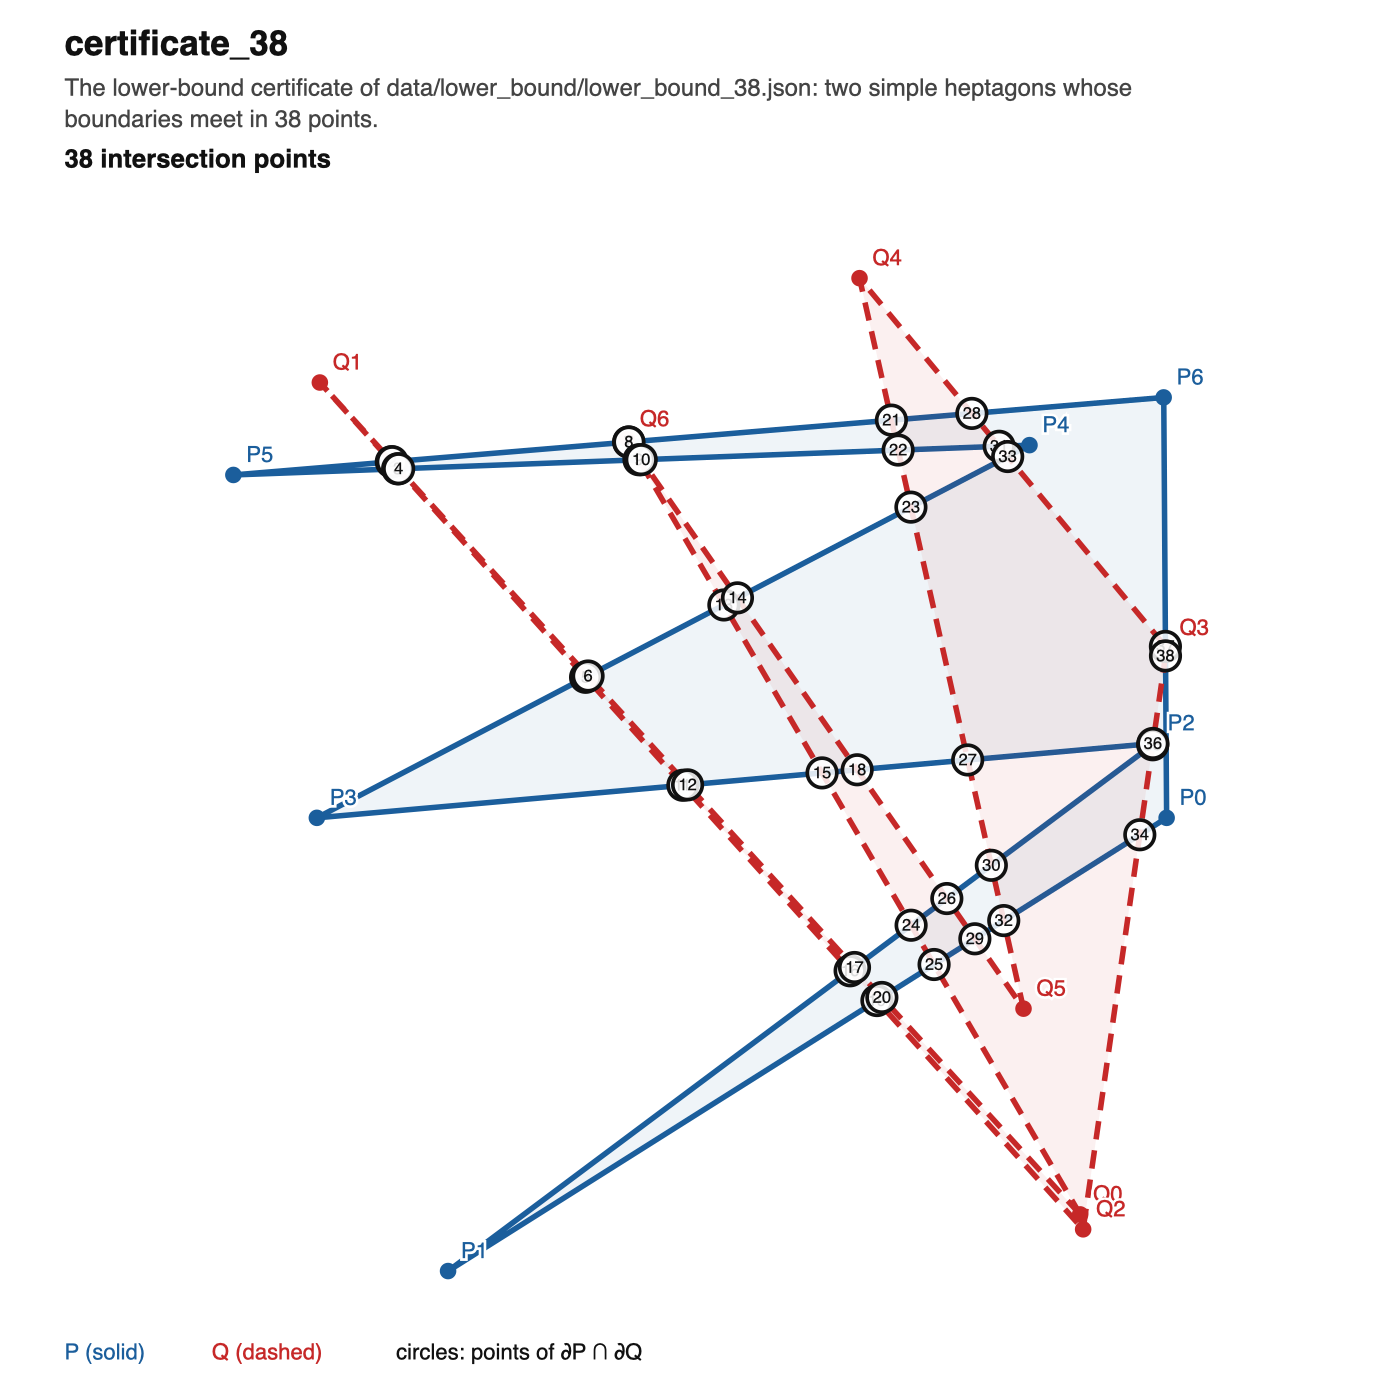
\includegraphics[width=\linewidth]{out/png/certificate_38.svg.png}
\par\smallskip{\footnotesize\texttt{certificate\_38}\\[1pt]computed count: \textbf{38}}
\end{minipage}
\caption{The lower-bound certificate. Every point of $\partial P\cap\partial Q$ is circled and numbered; there are \textbf{38}. This is the same configuration the Lean proof uses as its witness, read from the same JSON file.}
\end{figure}
\begin{figure}[p]\centering
\begin{minipage}[t]{0.45\textwidth}\centering
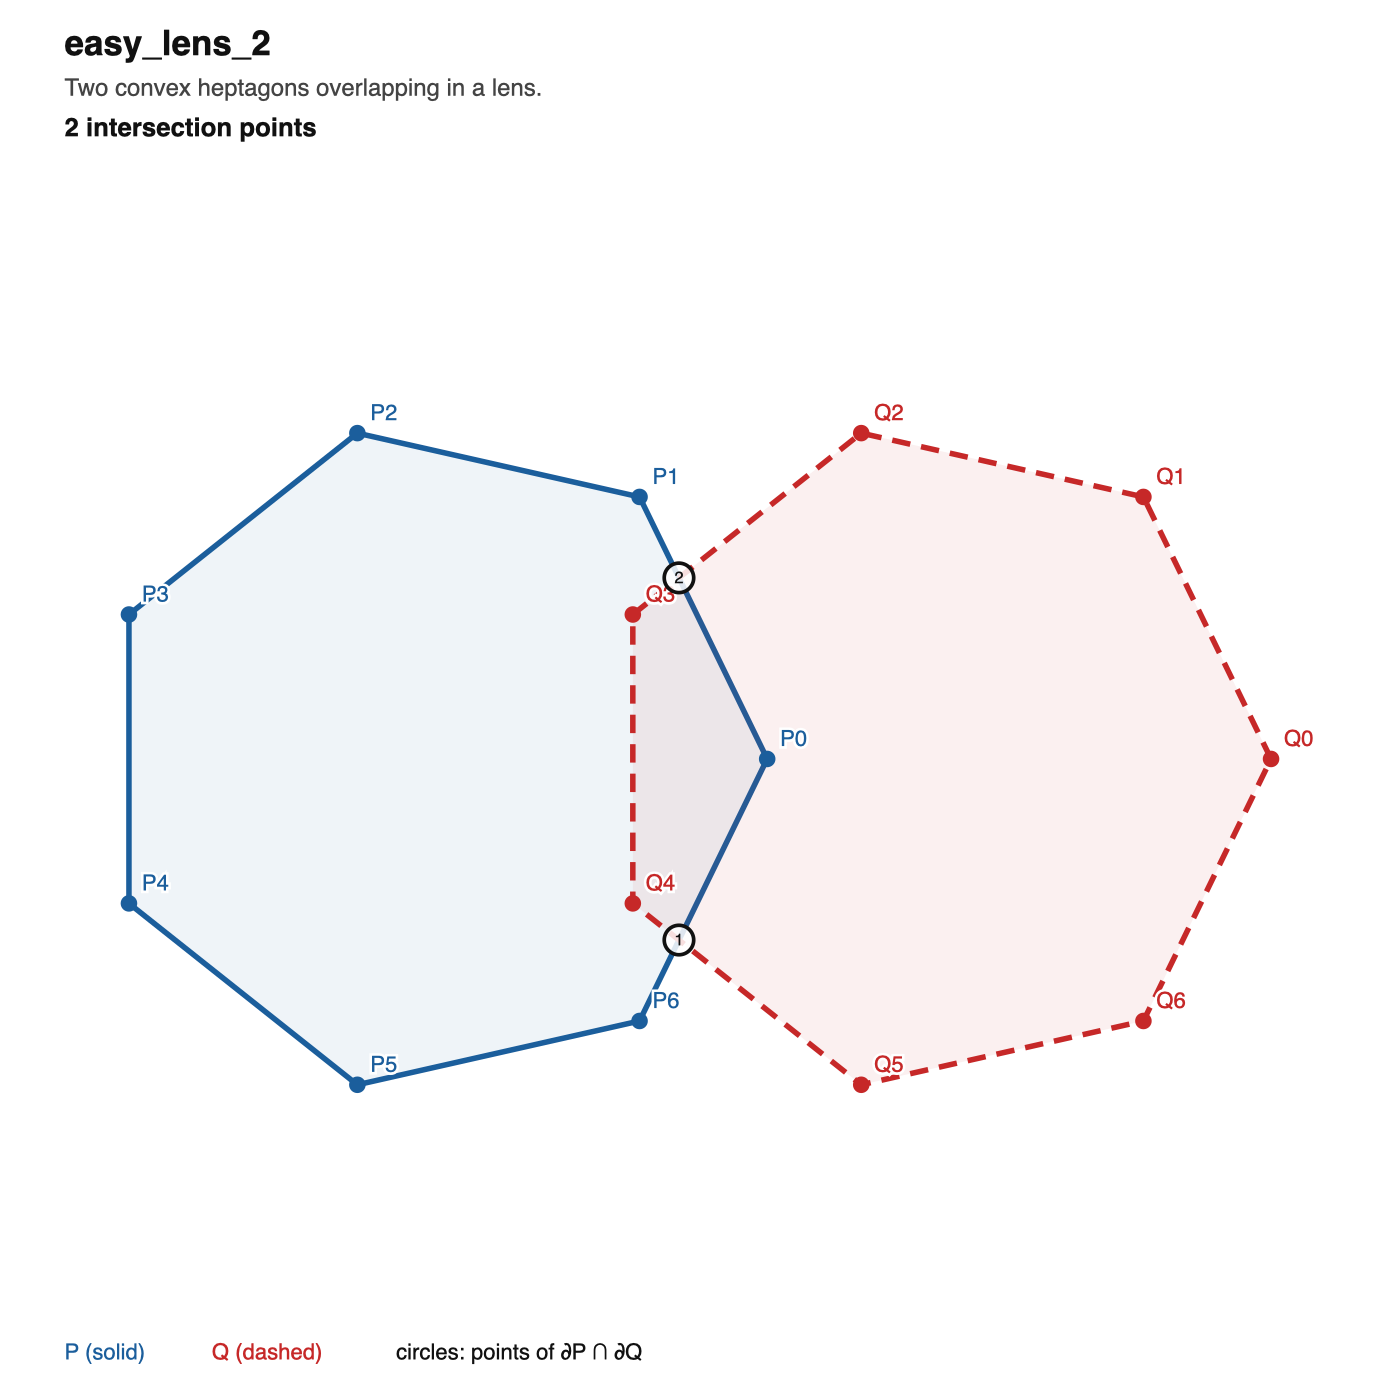
\includegraphics[width=\linewidth]{out/png/easy_lens_2.svg.png}
\par\smallskip{\footnotesize\texttt{easy\_lens\_2}\\[1pt]computed count: \textbf{2}}
\end{minipage}
\hfill
\begin{minipage}[t]{0.45\textwidth}\centering
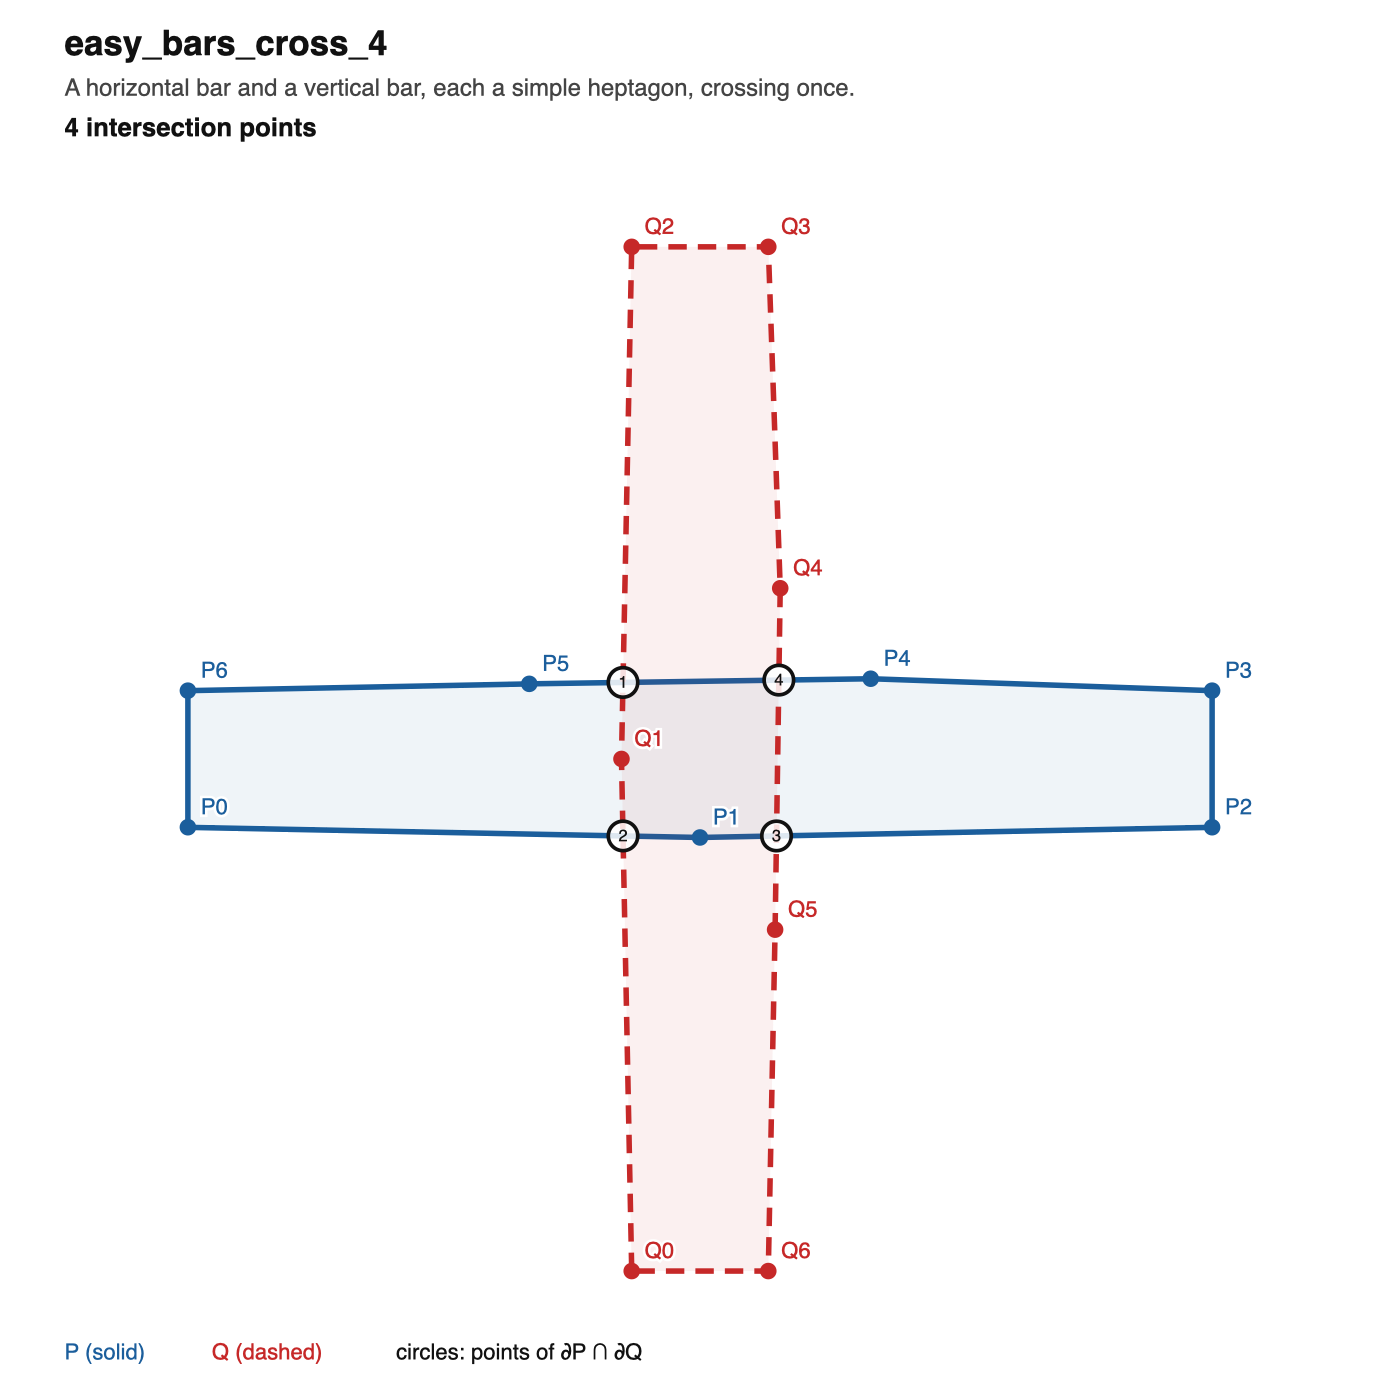
\includegraphics[width=\linewidth]{out/png/easy_bars_cross_4.svg.png}
\par\smallskip{\footnotesize\texttt{easy\_bars\_cross\_4}\\[1pt]computed count: \textbf{4}}
\end{minipage}
\par\bigskip
\begin{minipage}[t]{0.45\textwidth}\centering
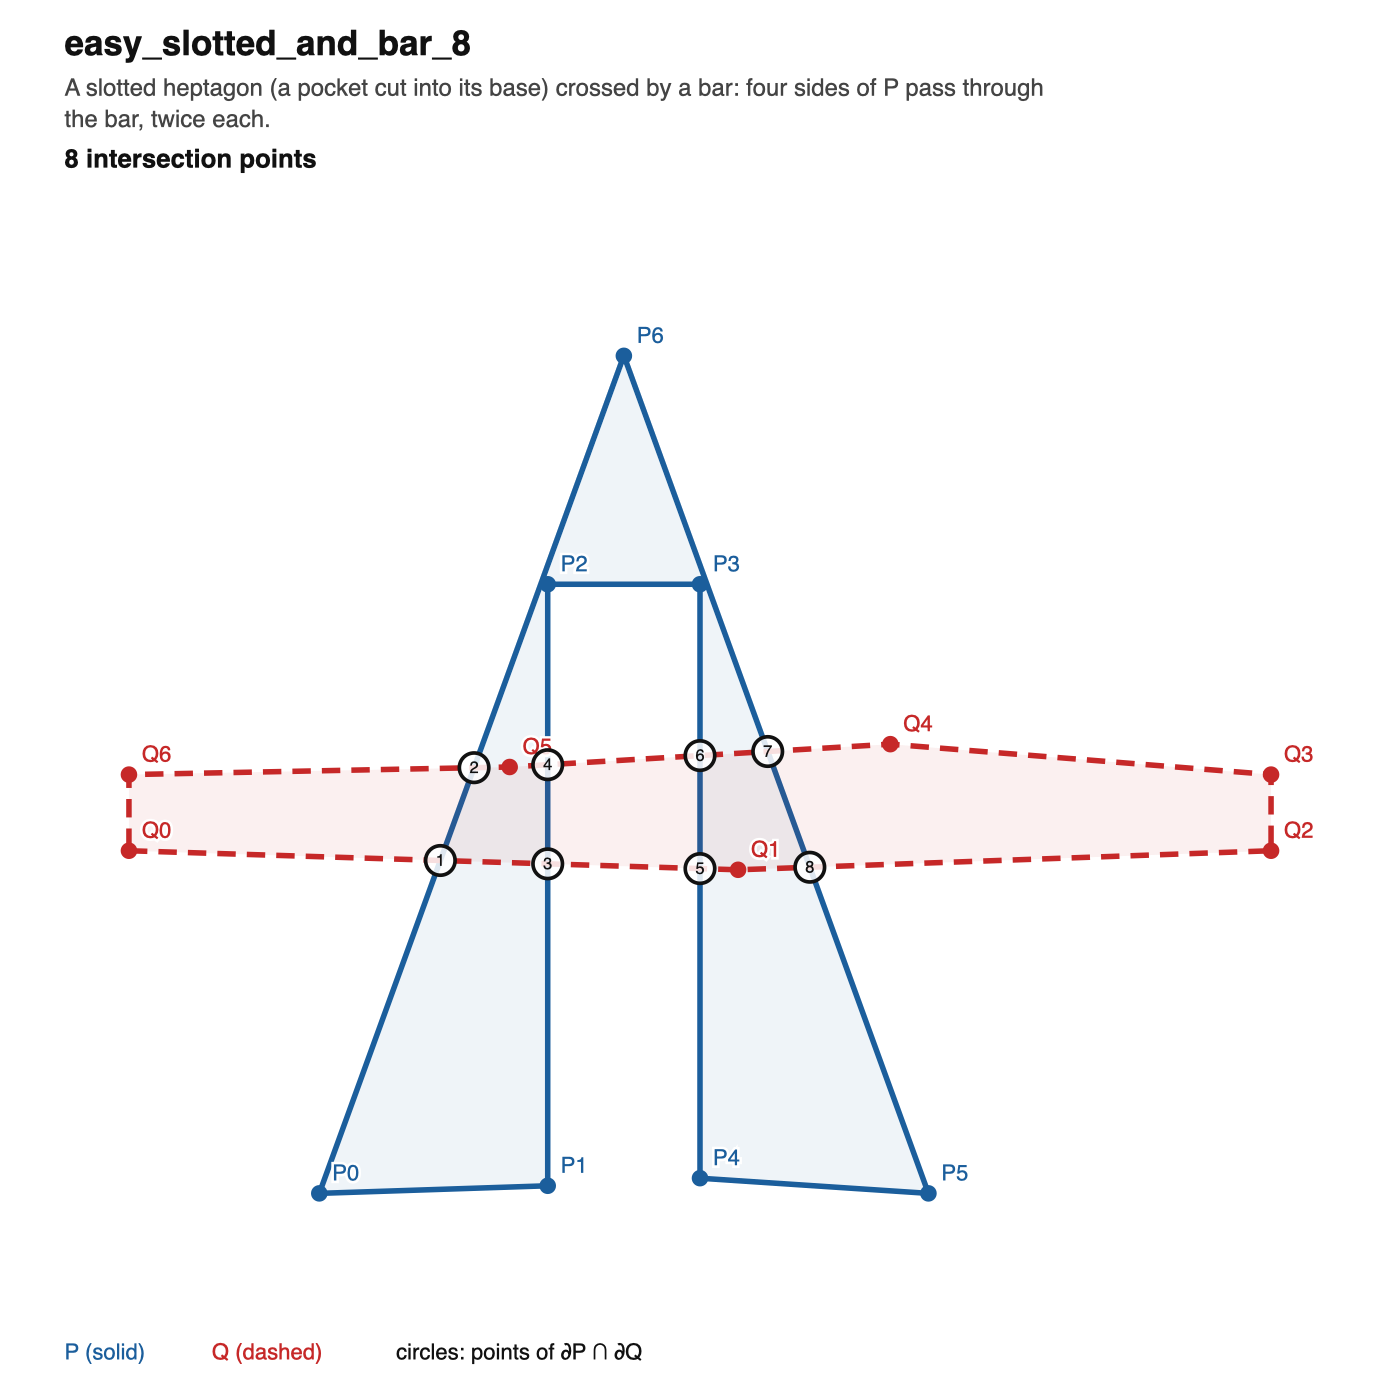
\includegraphics[width=\linewidth]{out/png/easy_slotted_and_bar_8.svg.png}
\par\smallskip{\footnotesize\texttt{easy\_slotted\_and\_bar\_8}\\[1pt]computed count: \textbf{8}}
\end{minipage}
\hfill
\begin{minipage}[t]{0.45\textwidth}\centering
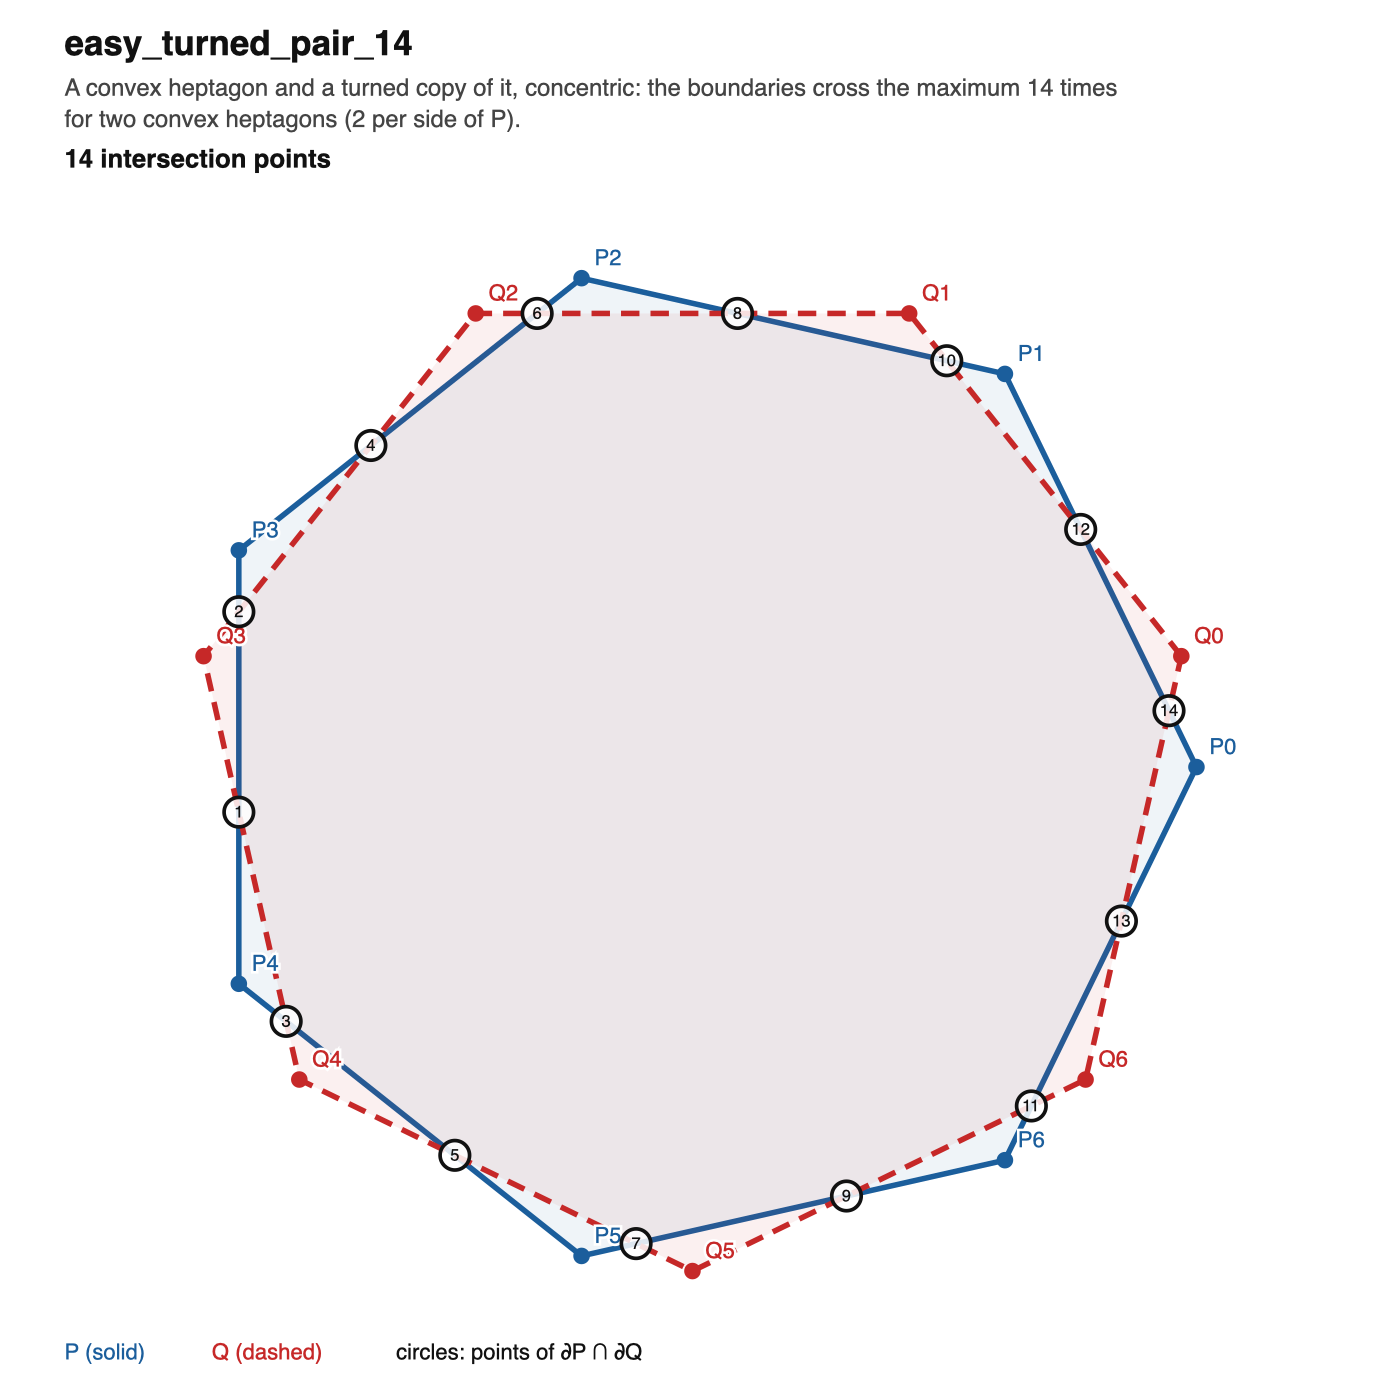
\includegraphics[width=\linewidth]{out/png/easy_turned_pair_14.svg.png}
\par\smallskip{\footnotesize\texttt{easy\_turned\_pair\_14}\\[1pt]computed count: \textbf{14}}
\end{minipage}
\par\bigskip
\caption{Sanity checks with answers you can see at a glance.}
\end{figure}
\begin{figure}[p]\centering
\begin{minipage}[t]{0.45\textwidth}\centering
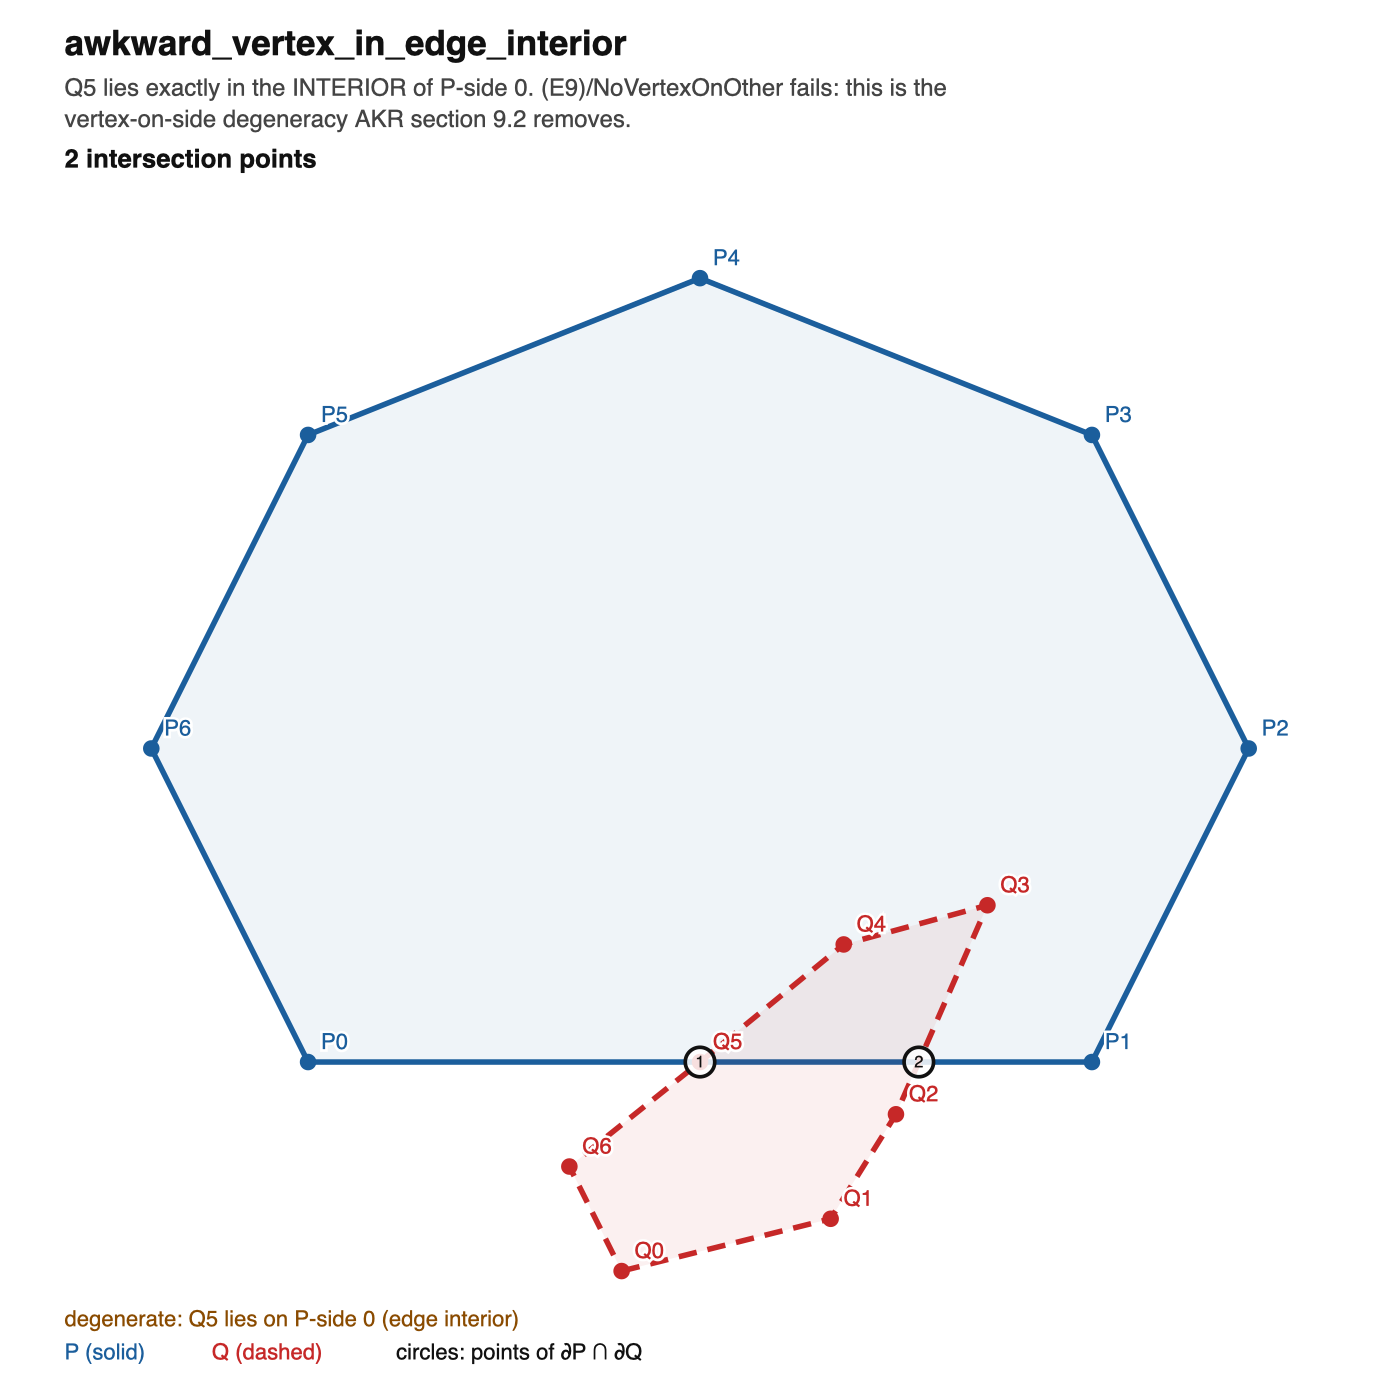
\includegraphics[width=\linewidth]{out/png/awkward_vertex_in_edge_interior.svg.png}
\par\smallskip{\footnotesize\texttt{awkward\_vertex\_in\_edge\_interior}\\[1pt]computed count: \textbf{2}}
\end{minipage}
\hfill
\begin{minipage}[t]{0.45\textwidth}\centering
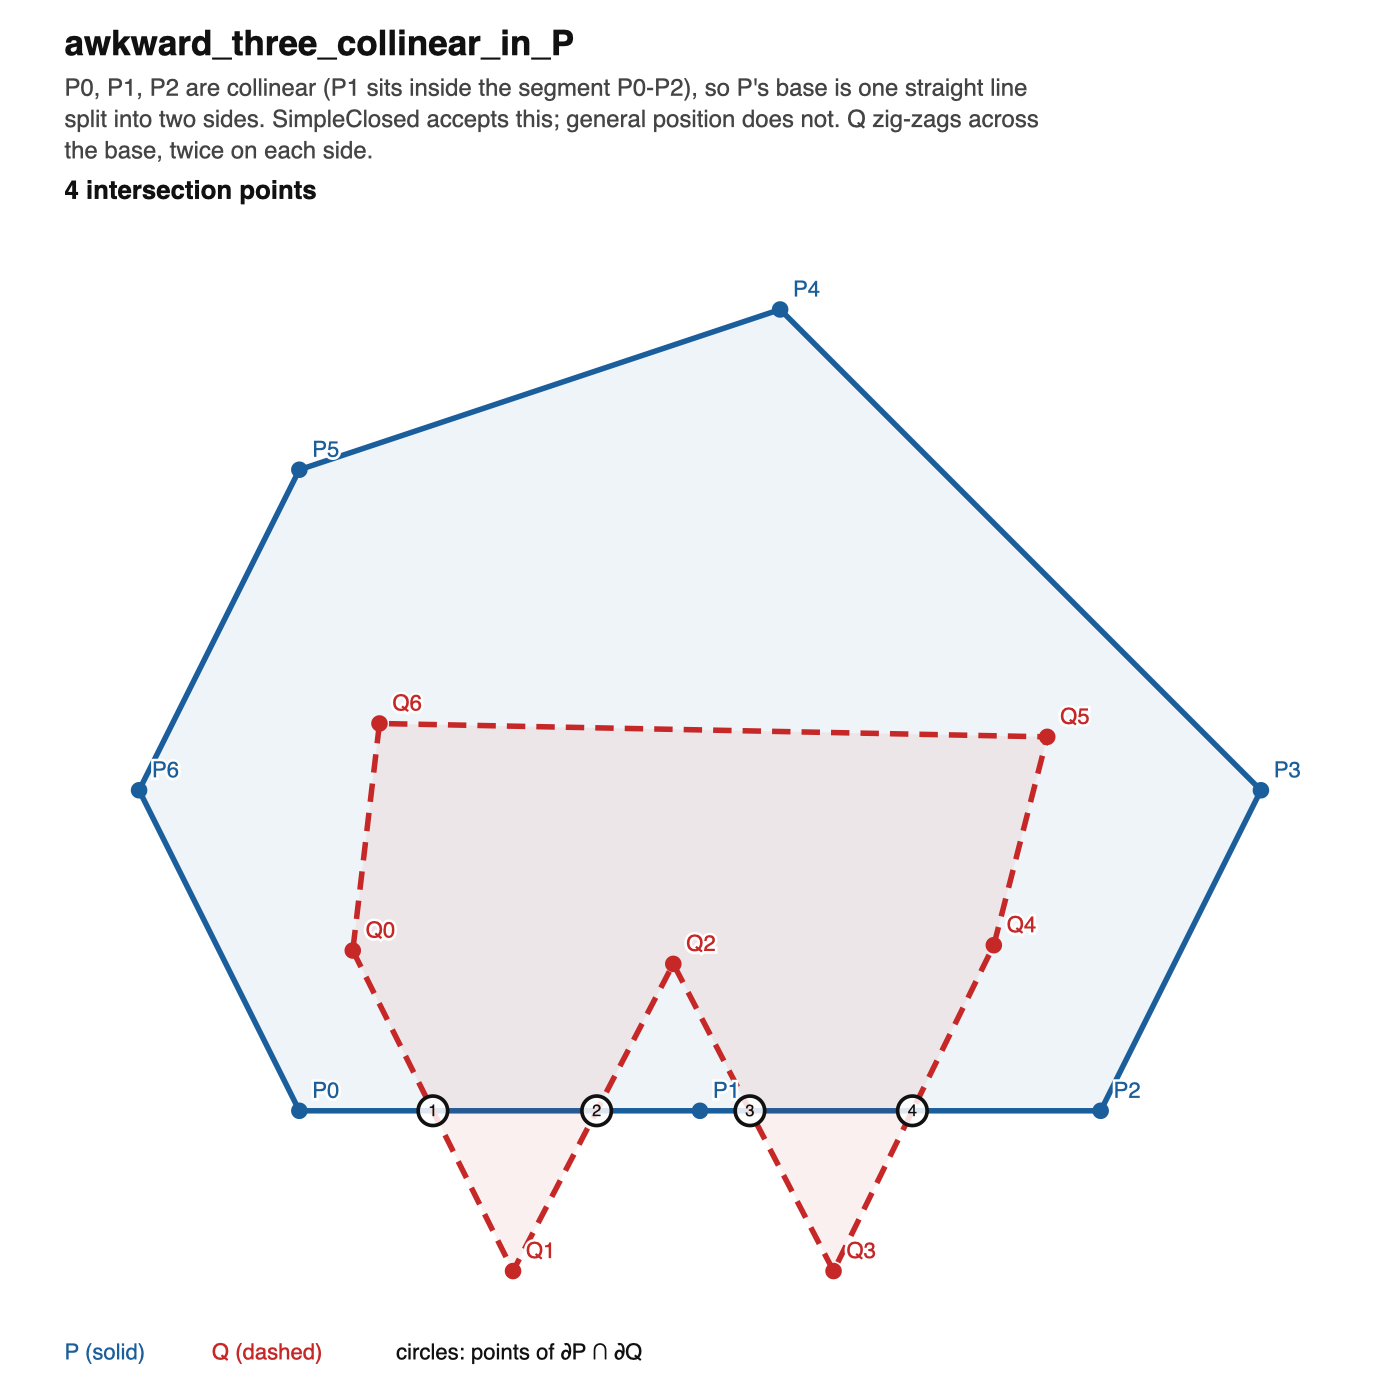
\includegraphics[width=\linewidth]{out/png/awkward_three_collinear_in_P.svg.png}
\par\smallskip{\footnotesize\texttt{awkward\_three\_collinear\_in\_P}\\[1pt]computed count: \textbf{4}}
\end{minipage}
\par\bigskip
\begin{minipage}[t]{0.45\textwidth}\centering
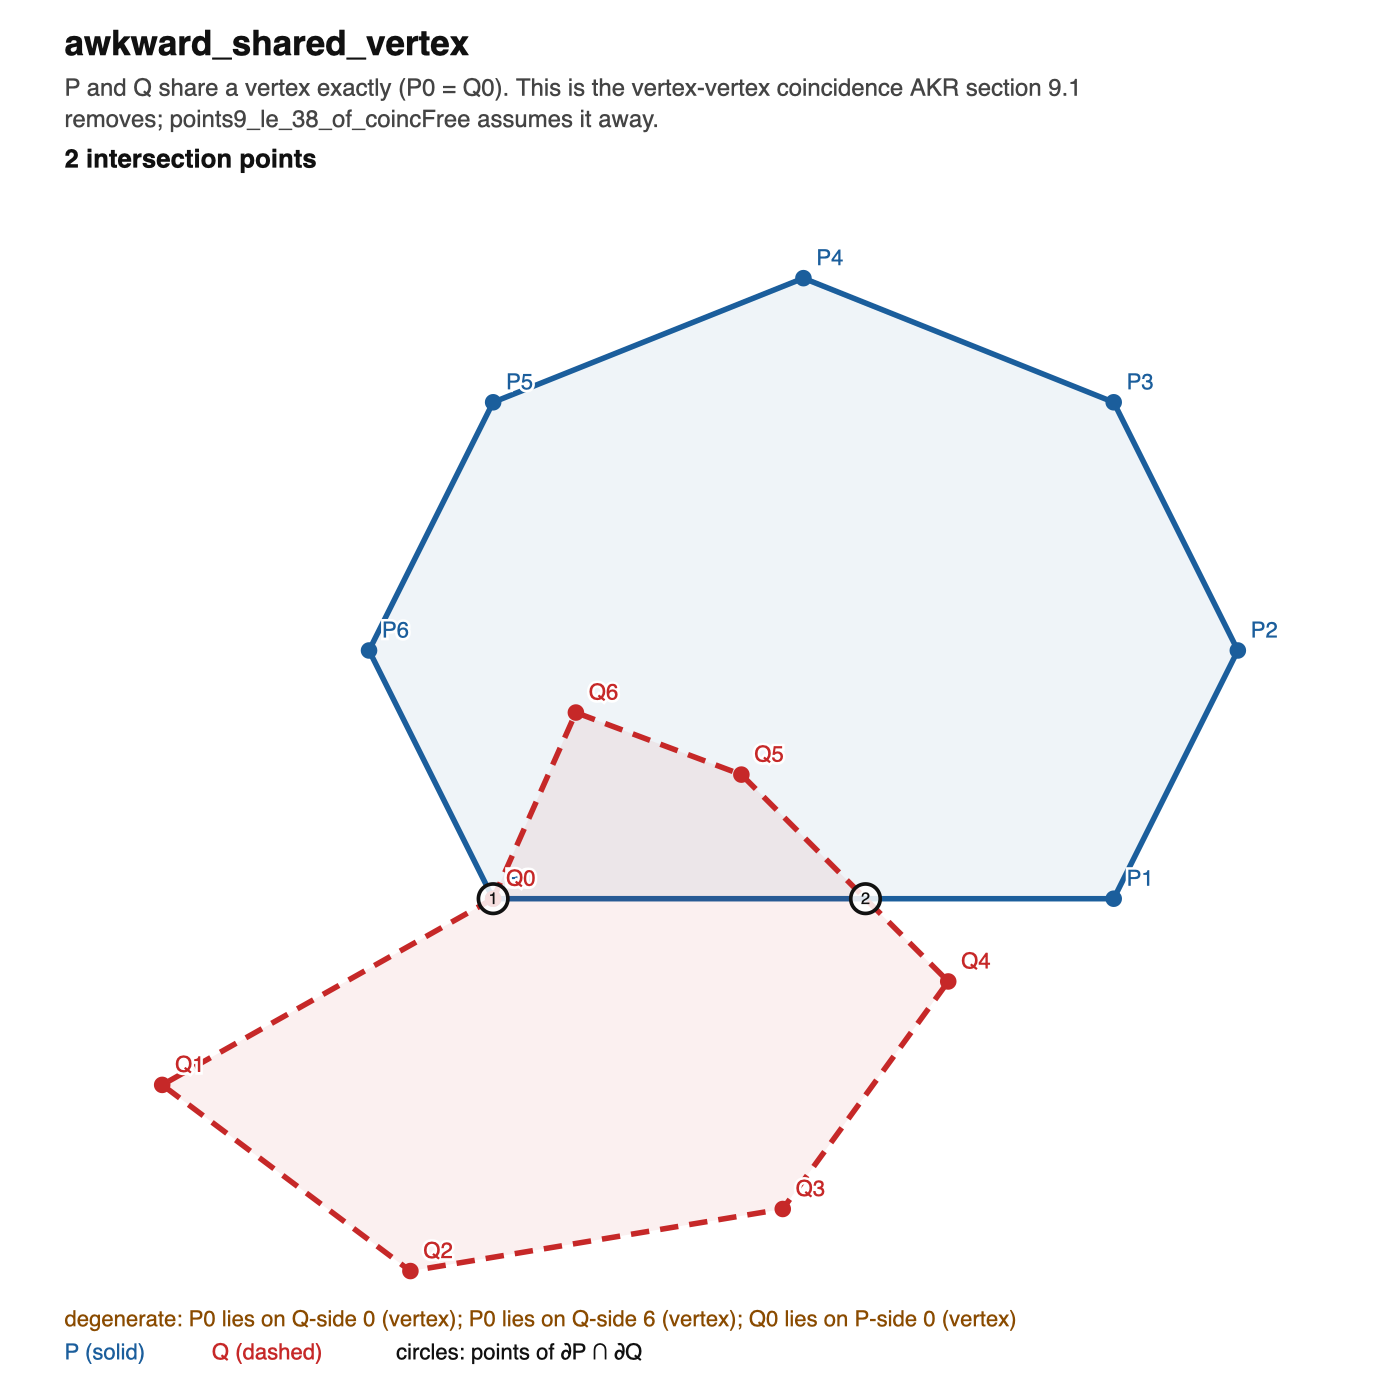
\includegraphics[width=\linewidth]{out/png/awkward_shared_vertex.svg.png}
\par\smallskip{\footnotesize\texttt{awkward\_shared\_vertex}\\[1pt]computed count: \textbf{2}}
\end{minipage}
\hfill
\begin{minipage}[t]{0.45\textwidth}\centering
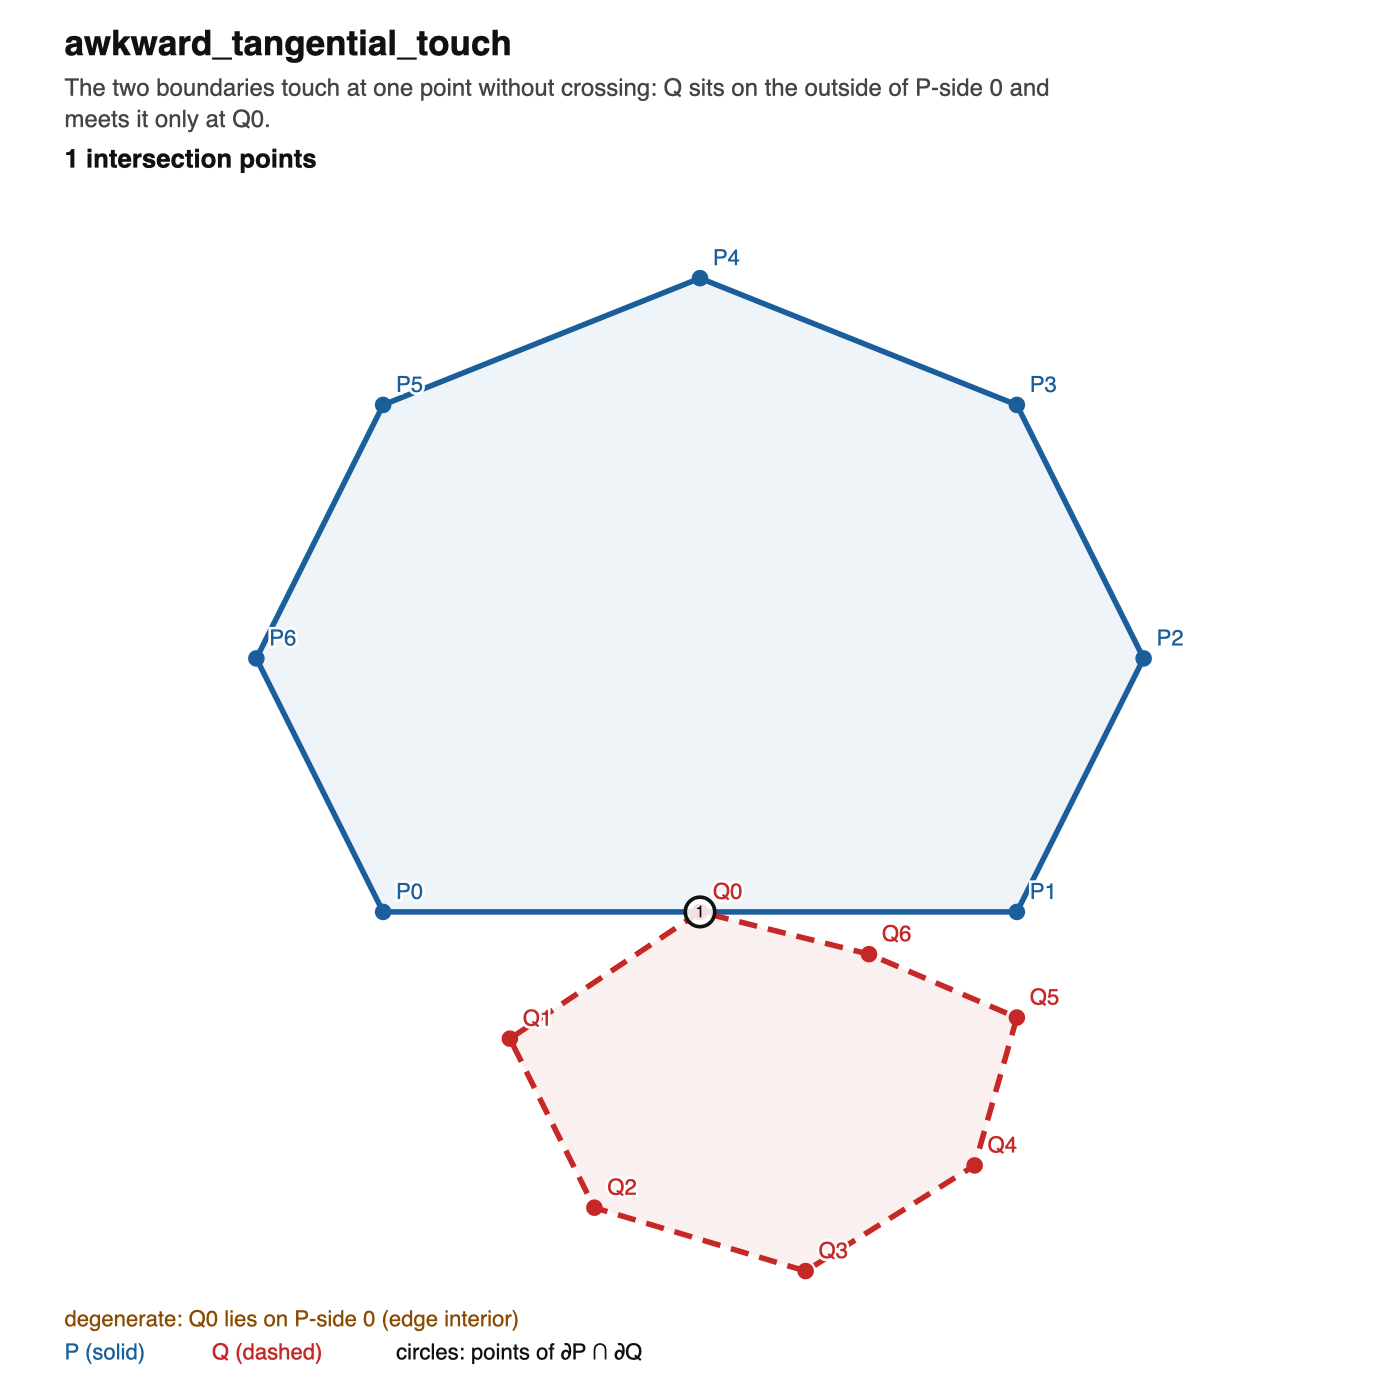
\includegraphics[width=\linewidth]{out/png/awkward_tangential_touch.svg.png}
\par\smallskip{\footnotesize\texttt{awkward\_tangential\_touch}\\[1pt]computed count: \textbf{1}}
\end{minipage}
\par\bigskip
\caption{Degeneracies that the theorem's hypotheses \emph{allow}, plus the one they exclude (\texttt{awkward\_shared\_vertex}).}
\end{figure}
\begin{figure}[p]\centering
\begin{minipage}[t]{0.45\textwidth}\centering
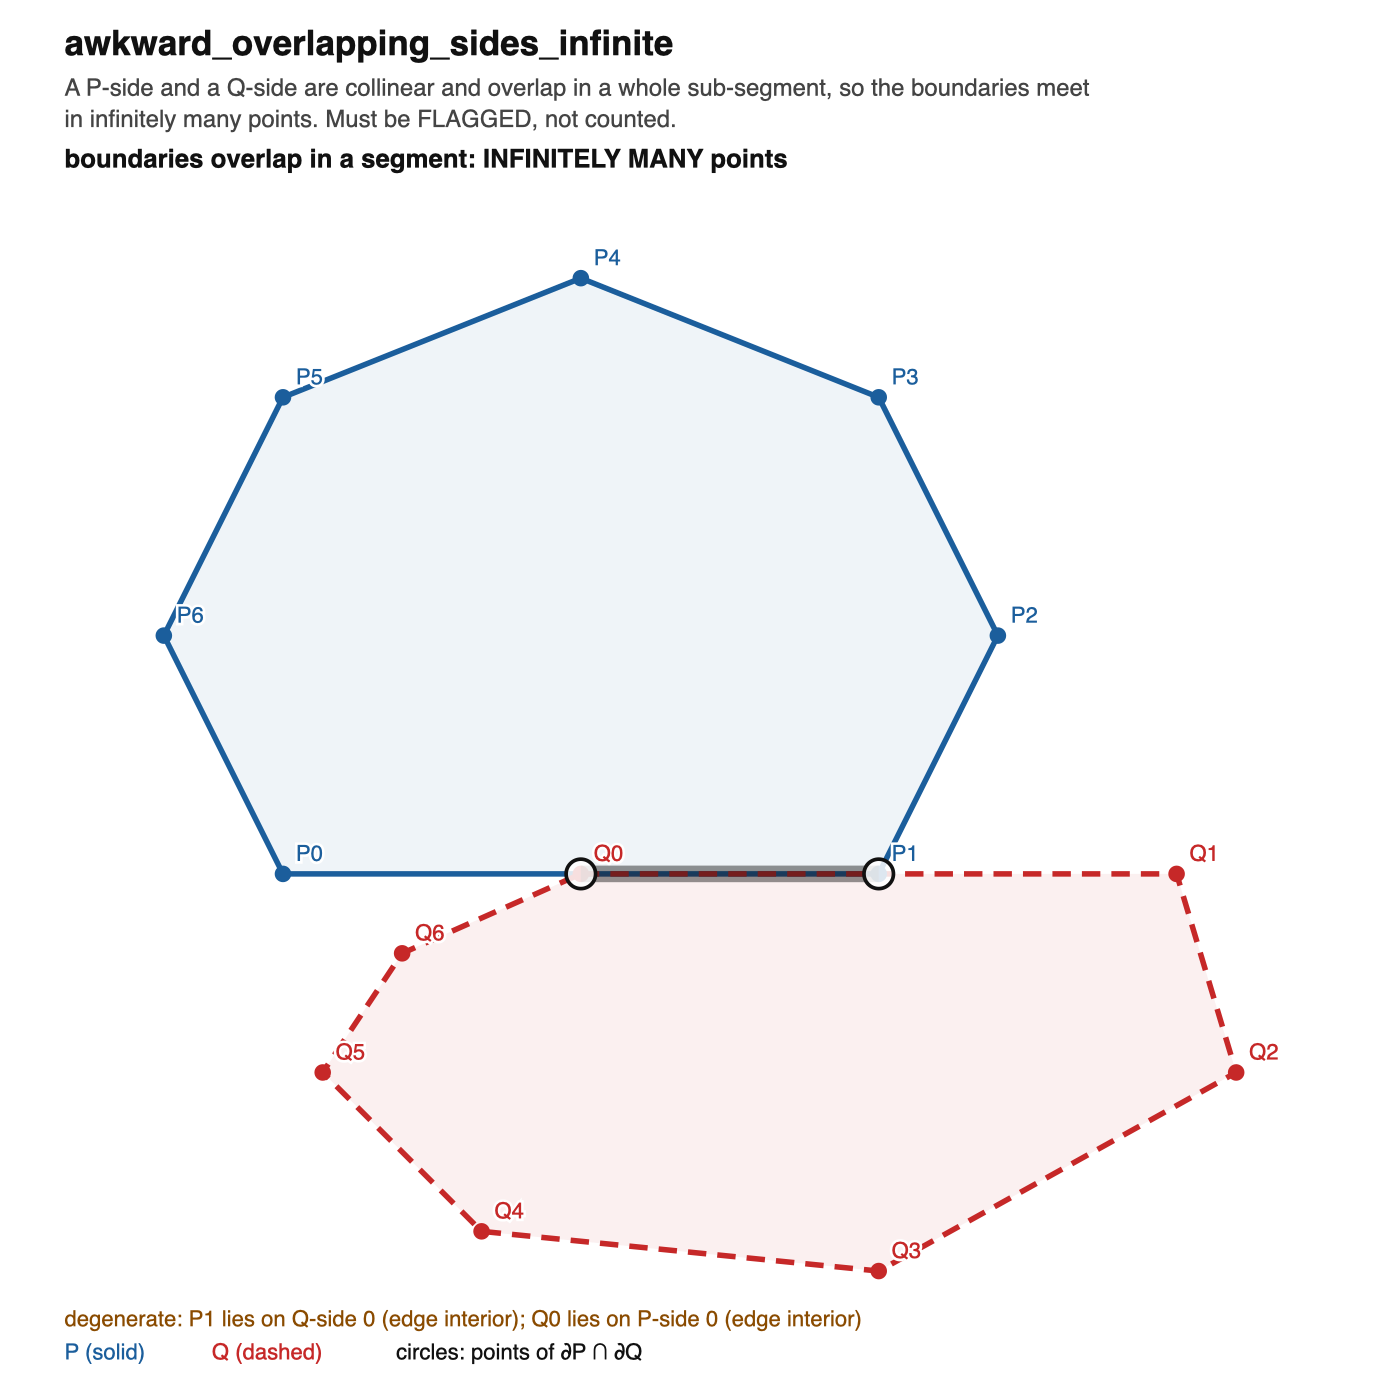
\includegraphics[width=\linewidth]{out/png/awkward_overlapping_sides_infinite.svg.png}
\par\smallskip{\footnotesize\texttt{awkward\_overlapping\_sides\_infinite}\\[1pt]computed count: \textbf{\textsc{infinite}}}
\end{minipage}
\hfill
\caption{The honest failure mode: two sides overlap in a whole sub-segment, so the intersection is genuinely infinite. It is flagged, not miscounted.}
\end{figure}


\section{Sabotage: does the checker ever say no?}

A verification that cannot fail proves nothing. If a check passes on this
repository, the first question is whether it would also pass on a broken one.
The repository answers this with controlled mutations: take a throwaway copy,
introduce one specific defect, and require that the check rejects it \emph{and
names the right reason}. A control copy with no defect must still be accepted,
so that ``rejects everything'' is not mistaken for rigour.

\paragraph{L4 first, because it is the one that is not about broken proofs.}
Every other test below breaks a \emph{proof}. L4 breaks a \emph{definition}.
The mutation changes one character in \code{lean/AKR9.lean}:

\begin{trustbox}
% generated by docs/audit/make_tables.py from scripts/negative-tests.sh
{\footnotesize\ttfamily\setlength{\parindent}{0pt}\raggedright
\mbox{}def~points9~(R~:~Pair9)~:~Set~($\mathbb{R}$~$\times$~$\mathbb{R}$)~:=~bdryP9~R~$\cap$~bdryQ9~R\\[4pt]
}{\footnotesize\itshape becomes\\[4pt]}
{\footnotesize\ttfamily\setlength{\parindent}{0pt}\raggedright
\mbox{}def~points9~(R~:~Pair9)~:~Set~($\mathbb{R}$~$\times$~$\mathbb{R}$)~:=~bdryP9~R~$\cup$~bdryQ9~R
}

\end{trustbox}

\noindent No proof text is touched. There is no \code{sorry}, no axiom, no
\code{native\_decide}; the mutated file is a Lean development about the union
of two boundaries instead of their intersection, a set that is not finite of
size at most 38. \Lfourreq

The test shows that the proofs depend on \code{points9} at least to the extent
that this change breaks them. It does not show that every unintended
definition would be rejected; mutation tests demonstrate rejection of the
particular mutations tested. \Lfourupshot

\paragraph{The three groups.}
\code{scripts/negative-tests.sh} has three groups. Group~N mutates the
evidence files (certificates, hashes, refutation proofs). Group~A mutates the
\emph{axiom log} and drives the repository's axiom checker over it --- these
need no Lean at all, because the checker is a log parser and can be tested the
way any parser is tested. Group~L is the four Lean-level mutations, L1--L4;
they require a real \code{lake build} of each mutated copy and are opt-in
behind a \code{--lean} flag.

\smallskip
\noindent Groups~A and~L were both run on 25~September~2026 (UTC), on the
author's machine, and both transcripts are committed. The two tables below are
generated from those transcripts.

\smallskip
\noindent One thing to know before reading them. \code{negative-tests.sh} can
print five verdicts --- \emph{accepted}, \emph{caught}, \textsc{not caught},
\textsc{not applied}, \textsc{wrongly rejected} --- and the generator that
builds these tables renders all five, so an absence of failures below reflects
the runs rather than the table. An earlier version of the generator
recognised only three of the five verdicts and would have dropped a failing
row; this was found and fixed before this document was built.

% generated by docs/audit/make_tables.py from out/negative_tests_A.log
\begingroup\small\setlength{\tabcolsep}{4pt}
\noindent\begin{tabular}{@{}lp{0.52\textwidth}r@{}}
\toprule
case & the mutation & verdict\\
\midrule
\texttt{A1} & complete clean log (control) & accepted\\
\multicolumn{3}{@{}p{0.97\textwidth}@{}}{\hspace{1.2em}\footnotesize\itshape nothing --- a complete, clean \#print axioms log}\\[2pt]
\texttt{A2} & wrapped axiom list (control) & accepted\\
\multicolumn{3}{@{}p{0.97\textwidth}@{}}{\hspace{1.2em}\footnotesize\itshape nothing --- but one axiom list is wrapped across three lines}\\[2pt]
\texttt{A3} & sorryAx in a headline theorem & \textbf{caught}\\
\multicolumn{3}{@{}p{0.97\textwidth}@{}}{\hspace{1.2em}\footnotesize\itshape a headline theorem's axiom list contains sorryAx}\\[2pt]
\texttt{A4} & headline lines absent & \textbf{caught}\\
\multicolumn{3}{@{}p{0.97\textwidth}@{}}{\hspace{1.2em}\footnotesize\itshape a log whose headline modules were never built: clean, but they never printed}\\[2pt]
\texttt{A5} & disallowed axiom (ofReduceBool) & \textbf{caught}\\
\multicolumn{3}{@{}p{0.97\textwidth}@{}}{\hspace{1.2em}\footnotesize\itshape a headline theorem depends on Lean.ofReduceBool (what native\_decide leaves)}\\[2pt]
\texttt{A6} & project-declared axiom & \textbf{caught}\\
\multicolumn{3}{@{}p{0.97\textwidth}@{}}{\hspace{1.2em}\footnotesize\itshape a headline theorem depends on a project-declared axiom}\\[2pt]
\texttt{A7} & no axiom output at all & \textbf{caught}\\
\multicolumn{3}{@{}p{0.97\textwidth}@{}}{\hspace{1.2em}\footnotesize\itshape a build log with no \#print axioms output whatsoever}\\[2pt]
\texttt{A8} & disallowed axiom in wrapped tail & \textbf{caught}\\
\multicolumn{3}{@{}p{0.97\textwidth}@{}}{\hspace{1.2em}\footnotesize\itshape a disallowed axiom hidden on the wrapped continuation line}\\[2pt]
\bottomrule
\end{tabular}\par\medskip
\noindent\textbf{\texttt{RESULT: 8 passed, 0 failed}}\ \ (\texttt{bash scripts/negative-tests.sh --groups A}, exit~0)
\endgroup


% generated by docs/audit/make_tables.py from results/validation/2026-09-24_negative_tests_L.log
\begin{trustbox}
\textbf{Group~L was run, and the transcript is committed.} The four Lean-level mutations --- a planted \code{sorry} (L1), a declared and used \code{axiom} (L2), a \code{native\_decide} (L3), and the changed definition described above (L4) --- each plant one defect in a copy-on-write clone of this repository, build the clone with a real \code{lake build}, and require the verifier to \emph{reject} it. The run is recorded at \texttt{results/validation/2026-09-24\_negative\_tests\_L.log}.
\par\smallskip{\footnotesize \texttt{date}~2026-09-25T01:37:04Z\quad \texttt{uname}~Darwin 24.6.0 arm64\quad \texttt{cmd}~NEGTESTS\_LAKE\_DIR=\$PWD/lean/.lake bash scripts/negative-tests.sh --lean --groups L}
\end{trustbox}
\begingroup\small\setlength{\tabcolsep}{4pt}
\noindent\begin{tabular}{@{}lp{0.52\textwidth}r@{}}
\toprule
case & the mutation & verdict\\
\midrule
\texttt{L1} & sorry in a dependency & \textbf{caught}\\
\multicolumn{3}{@{}p{0.97\textwidth}@{}}{\hspace{1.2em}\footnotesize\itshape a sorry planted three lemmas below a headline theorem; the log also shows \texttt{sorryAx}, so the mechanism under test is what fired}\\[2pt]
\texttt{L2} & declared axiom, used & \textbf{caught}\\
\multicolumn{3}{@{}p{0.97\textwidth}@{}}{\hspace{1.2em}\footnotesize\itshape an axiom was declared and used beneath a headline theorem; the log also shows \texttt{points9\_eq\_range\_ax}, so the mechanism under test is what fired}\\[2pt]
\texttt{L3} & native\_decide & \textbf{caught}\\
\multicolumn{3}{@{}p{0.97\textwidth}@{}}{\hspace{1.2em}\footnotesize\itshape a proof was closed by native\_decide (compiler, not kernel); the log also shows \texttt{ofReduceBool\textbar{}native\_decide}, so the mechanism under test is what fired}\\[2pt]
\texttt{L4} & definition changed (intersect-\textgreater{}union) & \textbf{caught}\\
\multicolumn{3}{@{}p{0.97\textwidth}@{}}{\hspace{1.2em}\footnotesize\itshape points9 redefined from an INTERSECTION to a UNION (no proof touched)}\\[2pt]
\bottomrule
\end{tabular}
\par\medskip
\noindent\textbf{\texttt{RESULT: 4 passed, 0 failed}}\ \ (\texttt{bash scripts/negative-tests.sh --lean --groups L})
\par\medskip\noindent Each of the four mutations was rejected by a build of a mutated copy. This shows that these four mutations are caught; it does not show that every defect would be.
 L4 bears on \S2 directly: no proof text was altered, only the \emph{definition} of \texttt{points9}, and the build failed.


\section{What the machine checked, and how to re-run it}

\begin{trustbox}
\begin{tabular}{@{}ll@{}}
\textit{working directory} & \textit{command}\\[2pt]
\code{lean/} & \code{lake exe cache get}\\
\code{lean/} & \code{lake build Headline 2>\&1 | tee ../headline-build.log}\\
repository root & \code{bash scripts/verify-all.sh --axiom-log headline-build.log}
\end{tabular}
\end{trustbox}

\noindent The first command downloads prebuilt Mathlib files for the revision
pinned in \code{lean/lake-manifest.json}; the second builds the headline
theorems; the third is the axiom check, which needs no Lean.
\medskip

{\sloppy
\noindent \code{lean/Headline.lean} declares nothing. It imports the four roots
of the live chain --- \code{MainTheorem}, \code{RealUpperBound}, \code{AKR9},
\code{Pair9Shift} --- and asks for the axiom lists of five declarations:\par}

\begin{trustbox}
\begin{Verbatim}[fontsize=\small]
#print axioms Heptagon.MainTheorem.isGreatest_38
#print axioms Heptagon.RealUpperBound.isGreatest_38_real
#print axioms Heptagon.AKR9.isGreatest_38_of_E9
#print axioms Heptagon.Pair9Shift.isGreatest_38_of_coincFree
#print axioms Heptagon.Pair9Shift.points9_le_38_of_coincFree
\end{Verbatim}
\end{trustbox}

\noindent Building that target builds the transitive closure of the four
roots --- 331 modules --- plus \code{Headline} itself: 332 modules of this
project, and no enumeration shard. Lake reports this as \hljobs\ \emph{jobs},
a count that also includes Mathlib's modules. The last two printed
declarations are the ones \S2 quotes. A bare \code{lake build} does
\emph{not} build them: the project's \code{defaultTargets} omits the \S9
modules, including \code{AKR9}, \code{Pair9Shift} and \code{Headline}.

\paragraph{The transcript of that command is committed.}
A full transcript of a local build of that target is in the repository, at
\hllogpath: \hllines\ lines, opening with a header that records the date
(\hllogdate), the machine, the Lean version, and the command. The header does
not record a commit. The Lean sources were last changed in commit
\code{a211140} (24~September~2026, 23:59 UTC), before this build, and have
not changed since; the transcript was committed in \code{b070c2f}.
Read out of that file:

\begin{itemize}
\item it ends with \code{Build completed successfully (\hljobs\ jobs).};
\item it carries \hldepends\ \code{depends on axioms} lines and one line for a
  declaration that depends on no axioms --- \hlparsed\ declarations in all ---
  and across them exactly \hlnaxioms\ distinct axioms appear: \code{propext},
  \code{Classical.choice} and \code{Quot.sound}. There is no fourth entry
  anywhere in the file;
\item \code{sorryAx} occurs \hlsorry\ times in it, and
  \code{Lean.ofReduceBool} --- what \code{native\_decide} would leave ---
  \hlnative\ times;
\item each of the six theorems the repository's checker demands printed an
  axiom line of its own. Five of the \code{\#print axioms} \emph{directives}
  that produce those lines sit in \code{lean/Headline.lean} at lines 45--49.
  The sixth, for \code{points\_le\_38\_of\_no\_vertex\_on\_boundary}, is a
  directive at \code{lean/AKR9.lean:420} --- the \emph{theorem} itself is
  stated at \code{lean/AKR9.lean:354} --- which is why that one axiom line
  appears about a thousand lines earlier in the log than the other five.
\end{itemize}

\noindent The repository's axiom checker
is a log parser that needs no Lean toolchain, and it can be pointed at that
file directly:

\begin{trustbox}
\centering\code{bash scripts/verify-all.sh --axiom-log}\\
\code{results/validation/2026-09-24\_headline\_build.log}
\end{trustbox}

\noindent It exits~0, and reports \hlparsed\ declarations parsed,
\hlbadaxioms\ of them using a disallowed axiom, and \hlheadlines\ headline
theorems confirmed. Its full output is committed at
\code{docs/audit/out/axiom\_check\_headline.log}. The transcript's own
provenance header, its six headline axiom lines, its last line, and the
checker's verdict on it are reproduced here:

% generated by docs/audit/make_tables.py from
%   results/validation/2026-09-24_headline_build.log
%   docs/audit/out/axiom_check_headline.log
\begingroup\footnotesize\ttfamily\setlength{\parindent}{0pt}\raggedright
\mbox{}\#~date~~:~2026-09-25T01:36:38Z\\
\mbox{}\#~uname~:~Darwin~24.6.0~arm64\\
\mbox{}\#~lean~~:~Lean~(version~4.33.1,~arm64-apple-darwin24.6.0,\\
\mbox{}~~~~~~~~~~~commit~819816b2e0a3bf405af45ae5c7af2491d8f5bee6,~Release)\\
\mbox{}\#~cmd~~~:~cd~lean~\&\&~lake~build~Headline\\
\mbox{}~~\dots\\
\mbox{}info:~AKR9.lean:420:0:~'Heptagon.AKR9.points\_le\_38\_of\_no\_vertex\_on\_boundary'~\\
\mbox{}~~~~depends~on~axioms:~[propext,~Classical.choice,~Quot.sound]\\[2pt]
\mbox{}info:~Headline.lean:45:0:~'Heptagon.MainTheorem.isGreatest\_38'~\\
\mbox{}~~~~depends~on~axioms:~[propext,~Quot.sound]\\[2pt]
\mbox{}info:~Headline.lean:46:0:~'Heptagon.RealUpperBound.isGreatest\_38\_real'~\\
\mbox{}~~~~depends~on~axioms:~[propext,~Classical.choice,~Quot.sound]\\[2pt]
\mbox{}info:~Headline.lean:47:0:~'Heptagon.AKR9.isGreatest\_38\_of\_E9'~\\
\mbox{}~~~~depends~on~axioms:~[propext,~Classical.choice,~Quot.sound]\\[2pt]
\mbox{}info:~Headline.lean:48:0:~'Heptagon.Pair9Shift.isGreatest\_38\_of\_coincFree'~\\
\mbox{}~~~~depends~on~axioms:~[propext,~Classical.choice,~Quot.sound]\\[2pt]
\mbox{}info:~Headline.lean:49:0:~'Heptagon.Pair9Shift.points9\_le\_38\_of\_coincFree'~\\
\mbox{}~~~~depends~on~axioms:~[propext,~Classical.choice,~Quot.sound]\\[2pt]
\mbox{}Build~completed~successfully~(3344~jobs).\\
\par\endgroup
\par\smallskip\noindent{\footnotesize Quoted from \texttt{results/validation/2026-09-24\_headline\_build.log} (83{,}020 lines): the provenance header, the six headline axiom lines (log lines 82448, 83015, 83016, 83017, 83018, 83019), and the final line~83020.}
\par\medskip\noindent{\footnotesize The repository's own axiom checker, run over that transcript (the command boxed above; exit~0) reports:}
\par\smallskip\begingroup\footnotesize\ttfamily\setlength{\parindent}{0pt}\raggedright
\mbox{}'depends~on~axioms'~lines~found~~~~~~~~~~:~408\\
\mbox{}declarations~parsed~~~~~~~~~~~~~~~~~~~~~~:~409\\
\mbox{}declarations~using~a~disallowed~axiom~~~~:~0\\
\mbox{}occurrences~of~sorryAx~~~~~~~~~~~~~~~~~~~:~0\\
\mbox{}distinct~axioms~~~~~~~~~~~~~~~~~~~~~~~~~~:~3\\
\mbox{}headline~theorems~confirmed~~~~~~~~~~~~~~:~6~of~6\\
\par\endgroup
\par\smallskip\noindent{\footnotesize\itshape AXIOM CHECK: CLEAN --- 409 declaration(s) reported their axioms; every one of the 3 distinct axioms used is among propext, Classical.choice, Quot.sound; sorryAx appears nowhere; all 6 headline theorems confirmed.}


\begin{trustbox}
\textbf{Six axiom lines are not six unconditional theorems.} They all carry the
number $38$ and they are not the same claim, so they are worth separating
before you read the list above.

\smallskip
\noindent Five of the six are statements about point sets in $\mathbb{R}^2$,
and they differ in their hypotheses:
\begin{itemize}
\item \code{points9\_le\_38\_of\_coincFree} and
  \code{isGreatest\_38\_of\_coincFree}: finiteness and no shared vertex --- the
  statement of \S2;
\item \code{points\_le\_38\_of\_no\_vertex\_on\_boundary} and
  \code{isGreatest\_38\_of\_E9}: the older, stronger hypothesis (E9), that no
  vertex of either polygon lies anywhere on the other's boundary; finiteness
  is then a consequence. Superseded by the two above;
\item \code{isGreatest\_38\_real}: general position, carried as a field of the
  structure \code{RConfig}.
\end{itemize}
Each assumes only the hypotheses written into its own statement. The
crossing-pair bound they rest on, \code{RawConfig.raw\_crossPairs\_card\_le\_38}
(\code{lean/RawConfig.lean:231}), takes a pair of point-set simple heptagons
with no general-position hypothesis.

\smallskip
\noindent \textbf{The sixth is a different animal.}
\code{MainTheorem.isGreatest\_38} (\code{lean/MainTheorem.lean:88}) is about a
different object --- integer-coordinate, orientation-level \code{Config}s ---
and it carries three explicit hypotheses which are what that route does
not itself prove: that every configuration has an
even crossing count, that none attains $42$, and that none attains $40$, the
last of these being the entire $13{,}003{,}620$-graph enumeration. Its own
doc-comment (\code{lean/MainTheorem.lean:45--48}) puts it plainly:

\smallskip
\noindent\emph{``So the honest reading of \code{isGreatest\_38} below is: `38
is the maximum crossing count over integer-coordinate, orientation-level
heptagon configurations, GIVEN the listed hypotheses.' Getting from there to
\code{f(7,7) = 38} needs the Jordan-curve step and the general-position
reduction, both external.''}

\smallskip
\noindent Note in the transcript above that this one has the \emph{shortest}
axiom list of the six --- \code{[propext, Quot.sound]}, with no
\code{Classical.choice}. That is a consequence of its being conditional, not a
sign that it is the strongest of them: an undischarged hypothesis costs no
axioms. Nothing in this document rests on it. The claim in \S1, the statement
in \S2 and the non-vacuity of \S\ref{sec:nonvac} are all the other route.
\end{trustbox}

\paragraph{Two figures in this section that the transcript does \emph{not}
establish.} It records no elapsed time, so the \textbf{11\,s} warm-build figure
is still only the repository's own assertion (\code{lean/README.md}) and you
should read it as that. And the log counts \emph{jobs}, not modules: the
\hljobs\ above is a job count, while the module count (331 in the closure of
the four roots, 332 with \code{Headline}) comes from a transitive-closure
computation over the \code{import} lines, repeated for this revision.

\paragraph{A correction, and what the axiom check really guards against.}
An earlier draft of this section asserted that \code{\#print axioms} prints
only when a module is actually recompiled, so that a warm rebuild ``replays
nothing and therefore prints nothing'' and only a cold build could produce this
evidence. \textbf{That was wrong}, and the committed transcript is what
demonstrates it: all \hlreplayed\ of its progress lines read \code{Replayed}
and not one reads \code{Built} --- it is a fully warm run --- and it
nevertheless carries every one of the \hldepends\ axiom lines, because Lake
replays the cached messages of the modules it does not recompile.

The trap the checker really guards against is a different one, and a worse one:
a log in which the headline theorems never appear \emph{at all}. That is what a
bare \code{lake build} produces here, because \code{defaultTargets} omits the
\S9 modules, so those theorems are never part of the build and never print.
Such a log exits~0 and looks clean while establishing nothing whatever about
the statements you care about. Test~A4 in \S4 is exactly that case and the
checker rejects it. Its requirement is not that the build was cold; it is that
each of the six named theorems printed an axiom line of its own.

\paragraph{Cost of a first build.} A fresh clone must first download
Mathlib (the Lean mathematical library, pinned here at tag \code{v4.33.1})
before any of this project's own code compiles. The repository records about
1.4\,GB in \code{lean/.lake} after a cold build, measured before later modules
were added, so treat it as a lower bound. On the GitHub-hosted runners of
\S\ref{sec:ci} (2 cores) the headline build step took about 32 minutes in the
second run.

\section{Recorded CI builds}\label{sec:ci}

The evidence in \S\S2--5 was produced on the author's computer. The repository
also has a GitHub Actions workflow (\code{.github/workflows/verify.yml}) that,
on each push to the main branch, checks out the repository on a
GitHub-hosted runner, installs the pinned Lean toolchain, fetches prebuilt
Mathlib files, builds the \code{Headline} target, and runs the axiom check
and the group-A tests of \S4. Two runs are recorded, both passing:

\begin{trustbox}
\small
\begin{tabular}{@{}lll@{}}
\textit{run} & \textit{commit} & \textit{started (UTC), duration}\\[2pt]
\code{36086080499} & \code{b78f372} & 25 Sep 2026 02:23, 40\,min 54\,s\\
\code{36089101301} & \code{e984888} & 25 Sep 2026 03:07, 35\,min 05\,s
\end{tabular}

\smallskip
{\footnotesize Both on \code{ubuntu-latest}, 2 cores, 7.8\,GiB. Both commits
have the Lean sources of \code{a211140}. Run pages are at\\
\texttt{github.com/NewYorkImperialist/heptagon-intersections/actions/runs/<run>}.}
\end{trustbox}

\noindent What the first run reported, quoted from the extract committed at
\code{docs/audit/out/ci\_run.log}:

\begin{trustbox}
\begin{Verbatim}[fontsize=\small]
lean/lean-toolchain pins: leanprover/lean4:v4.33.1
Build completed successfully (3344 jobs).
OK: 0 occurrences of sorryAx
   axiom-check: declarations parsed              : 409
   axiom-check: distinct axioms                  : 3
   axiom-check: headline theorems confirmed      : 6 of 6
   AXIOM CHECK: CLEAN
RESULT: 8 passed, 0 failed          (the group-A tests)
\end{Verbatim}
\end{trustbox}

\noindent The second run reported the same figures; its extract is
\code{docs/audit/out/ci\_run\_2.log}. They agree with the local transcript of
\S5: the same job count, the same 409 declarations, the same six theorems and
the same three axioms.

\paragraph{The project's modules were compiled, not restored.} Lake can
restore a previous build and replay its stored messages, which look the same
as freshly produced ones. The workflow does not cache \code{lean/.lake/build}.
In each run, Lake's progress output has 346 lines marked \emph{Built} and none
marked \emph{Replayed}: 332 are this project's modules (the whole
\code{Headline} closure) and 14 are jobs building Mathlib's \code{cache}
tool. Mathlib itself is fetched prebuilt for the pinned revision.

\paragraph{What these runs do and do not show.} They record that the committed
workflow passed at those two revisions on a machine not controlled by the
author. The workflow itself is written by the repository owner, so the runs
show what that workflow checks, and they do not cover later changes to the
repository. They do not run the Lean mutation tests L1--L4 of \S4 (an opt-in
job, not run; those results come from the local transcript), and they build
the 332-module headline closure, not all 1{,}779 declared libraries. They are
not a review of the mathematics or of the formal statements.

\paragraph{Access.} As of 4~October~2026 the repository is private (checked
with the GitHub command-line tool). The run pages and their artifacts are
visible only to people with access to the repository, and the artifacts expire
90 days after each run.

\section{Non-vacuity: the hypotheses can be met, and the bound is attained}\label{sec:nonvac}

{\sloppy
A conditional theorem whose hypotheses are contradictory is vacuously true and
says nothing. An upper bound nobody attains is not a maximum. Both failure modes
are closed explicitly at the end of \code{lean/Pair9Shift.lean}, by a single
bundled declaration, \code{nonVacuity}, in the \code{Heptagon.Pair9Shift}
namespace.\par}

% generated by docs/audit/make_tables.py -- do not edit by hand
\noindent{\footnotesize\ttfamily lean/Pair9Shift.lean:5296}\par\smallskip
{\footnotesize\ttfamily\setlength{\parindent}{0pt}\raggedright
\mbox{}theorem~nonVacuity~:\\[-1pt]
\mbox{}~~~~Nonempty~AKR9.Pair9\\[-1pt]
\mbox{}~~~~$\land$~(points9~AKR9.certPair9).Nonempty\\[-1pt]
\mbox{}~~~~$\land$~(points9~AKR9.certPair9).Finite\\[-1pt]
\mbox{}~~~~$\land$~($\forall$~v~j~:~Fin~7,~AKR9.certPair9.V~(pP~v)~$\ne$~AKR9.certPair9.V~(pQ~j))\\[-1pt]
\mbox{}~~~~$\land$~AKR9.NoVertexOnOther~AKR9.certPair9\\[-1pt]
\mbox{}~~~~$\land$~(points9~AKR9.certPair9).ncard~=~38\\[-1pt]
\mbox{}~~~~$\land$~$\lnot$~(points9~AKR9.certPair9).ncard~$\le$~37\\[-1pt]
\mbox{}~~~~$\land$~(38~:~$\mathbb{N}$)~$\in$~attainedCoincFree\\[-1pt]
\mbox{}~~~~$\land$~(39~:~$\mathbb{N}$)~$\notin$~attainedCoincFree\\[-1pt]
\mbox{}~~~~$\land$~IsGreatest~attainedCoincFree~38~:=\\[-1pt]
\mbox{}~~$\langle$pair9\_nonempty,~certPair9\_points9\_nonempty,~certPair9\_finite,\\[-1pt]
\mbox{}~~~certPair9\_coincFree,~certPair9\_noVertexOnOther,~AKR9.certPair9\_ncard,\\[-1pt]
\mbox{}~~~certPair9\_not\_le\_37,~mem\_attainedCoincFree\_38,~not\_mem\_attainedCoincFree\_39,\\[-1pt]
\mbox{}~~~isGreatest\_38\_of\_coincFree$\rangle$\\[-1pt]
}
\par\medskip\noindent Ten clauses, in order:
\begin{enumerate}[leftmargin=2.1em,label=\textbf{(\arabic*)}]
\item \code{Pair9} is inhabited: the two \code{SimpleClosed} hypotheses of \S2 are satisfiable at all. Without this the whole theory could be about an empty type.
\item The witness's intersection set is non-empty.
\item It is \emph{finite} --- so \code{ncard} is the real cardinality. On an infinite set \code{ncard} returns $0$, which would make the bound $\le 38$ true and meaningless; this clause closes that door. (Clause~(6) already implies it, for exactly that reason; it is stated separately for the reader.)
\item The witness satisfies \code{hcoinc}: it shares no vertex. The hypothesis of the theorem is not contradictory.
\item The witness also satisfies the \emph{stronger} condition \code{NoVertexOnOther} --- no vertex anywhere on the other boundary.
\item Its count is exactly $38$: \textbf{the bound is attained}.
\item $\le 37$ is \emph{false} there: \textbf{the bound is not slack}. One less is provably wrong, so $38$ is the right constant and not an artefact of a lossy estimate. (Immediate from~(6); stated because it is the thing a reader wants to see said.)
\item $38$ is an attained value.
\item $39$ is \emph{not} attained.
\item $38$ is the greatest attained value.
\end{enumerate}
\par\medskip\noindent These are ten clauses, not ten logically independent facts: (6) is the sharpest of them and already implies (3) and (7). The content is not the number of clauses but the fact that \textbf{(2)--(7) all hold of the \emph{same} configuration}, \code{AKR9.certPair9}. Checking hypotheses one at a time would not rule out a theorem whose hypotheses are each satisfiable but jointly contradictory; a single shared witness does. That is precisely the failure mode an absent human reviewer would be looking for, and the declaration's own doc-comment says so.
\par\medskip\noindent A companion records that the maximum is \emph{unique} --- any $n$ that is a greatest attained value equals $38$:\par\smallskip
\noindent{\footnotesize\ttfamily lean/Pair9Shift.lean:5272}\par\smallskip
{\footnotesize\ttfamily\setlength{\parindent}{0pt}\raggedright
\mbox{}theorem~isGreatest\_attainedCoincFree\_unique~\{n~:~$\mathbb{N}$\}\\[-1pt]
\mbox{}~~~~(h~:~IsGreatest~attainedCoincFree~n)~:~n~=~38~:=\\[-1pt]
\mbox{}~~h.unique~isGreatest\_38\_of\_coincFree\\[-1pt]
}


\section{What is not proved}\label{sec:notproved}

\paragraph{$f(7,7)=38$ is not a Lean theorem.} What is kernel-checked is the
statement in \S2: the bound $38$ for simple heptagons that share no vertex and
whose boundaries meet in finitely many points, with $38$ attained. Finiteness
is a hypothesis, not a conclusion; the last row of \S3 is a configuration
where it fails. The doc-comment on the theorem says the same: ``\emph{This is
not \code{f(7,7) = 38}, and it is not all of AKR \S9.}''

\paragraph{The vertex-coincidence reduction.} The reference is E.~Ackerman,
B.~Keszegh and G.~Rote, \emph{An almost optimal bound on the number of
intersections of two simple polygons}, Discrete Comput.\ Geom.\ \textbf{68}
(2022) 1049--1077; \S9 appears only in this journal version. Their \S9 shows
that degenerate cases --- a vertex of one polygon on the boundary of the other
--- can be removed without decreasing the number of intersection points. It
has two parts. \S9.2's part, a vertex in the \emph{interior} of a side, is
\emph{proved here} in Lean, by the project's own argument; that is what
\code{points9\_le\_38\_of\_coincFree} adds over its (E9) predecessor. \S9.1's
part, a vertex \emph{equal} to a vertex of the other polygon, is not proved
here. To obtain $f(7,7)=38$ one needs:
\begin{enumerate}
\item[(a)] \emph{kernel-checked:} the statement of \S2;
\item[(b)] \emph{from an external theorem:} the reduction of AKR \S9.1, that
  every pair can be replaced by one sharing no vertex without decreasing the
  number of intersection points;
\item[(c)] \emph{not settled in this project:} that the replaced pair is again
  simple in the sense of \S2 and again has finite intersection, as \S2's
  hypotheses require. We have not found either stated explicitly in AKR \S9.
  The project has a kernel-checked lemma that simplicity survives every
  sufficiently small linear motion of the vertices
  (\code{SimplicityStable.heptagon\_simplicity\_stable\_linear}), and
  unreviewed pen-and-paper notes on choosing the \S9.1 directions so that the
  intersection stays finite, but it has not assembled these with \S9.1 into a
  proof of the reduction for these definitions.
\end{enumerate}
Using a published theorem does not by itself make an argument incomplete;
the qualification here is item~(c).

\paragraph{Points the project noted in AKR \S9.} Two points arose while
working on \S9, recorded here because they bear on how much of \S9 can be
cited unchanged. They concern the procedure as printed, not the truth of the
theorem. First, \S9.2 moves the endpoints of a side along the lines of the
adjacent sides; when two consecutive sides are collinear, a configuration the
definitions of \S2 allow, the printed description does not determine the
move, and the project uses a different (``tilted'') shift. Second, the
criterion stated in \S9.1 for choosing perturbation directions does not, as
written, exclude directions that make the perturbed intersection infinite; an
additional condition, which AKR may regard as implicit, is needed. The project's
supplements are its own and are not reviewed. These points are documented in
\code{docs/verification-status.md}, rows 60--62.

\paragraph{Review status.} No independent review of the mathematics, the Lean
development or the Python tools has been completed. The project's records
(\code{docs/verification-status.md}, row~18) note that a colleague began
reading an earlier dependency manifest in September 2026, and record no
findings from that reading. Human review still matters for the statement and
definitions (\S2), for the external reduction and its applicability (above),
and for the connection between this document and the code that was checked
(\S\S2 and~5).

\paragraph{The gallery.} The gallery in \S3 is a Python \emph{transcription}
of the Lean predicates, checked against them by hand and annotated with line
numbers. It is evidence that the definitions compute what one expects on ten
examples, not a proof that the Python and the Lean agree.

{\sloppy\paragraph{Earlier gaps, now closed.} An earlier draft listed two further
items. That the \S5 build figures had no committed transcript is no longer
true: the transcript is at \hllogpath, and the axiom checker can be run over it
without Lean. That group~L of the mutation suite had never been run in a
recorded way is no longer true either: it was run, its transcript is
committed, and \S4 reports each case.\par}

\appendix
\section{The statement surface, verbatim and complete}

All \ndecls\ declarations extracted by \code{docs/audit/extract\_lean.py},
unedited, with file and line. The six that carry the content appear in \S2;
these are the rest, and the full text of those six.

% Verbatim Lean excerpts, LaTeX-escaped
% generated by docs/audit/extract_lean.py -- do not edit by hand
% requires lean_preamble.tex

\begin{leandecl}{pP}{lean/ResidualSymBase.lean}{23}
\leanline{def pP (i : Fin 7) : Fin 14 := $\langle$i.val, by omega$\rangle$}
\end{leandecl}

\begin{leandecl}{pQ}{lean/ResidualSymBase.lean}{26}
\leanline{def pQ (i : Fin 7) : Fin 14 := $\langle$7 + i.val, by omega$\rangle$}
\end{leandecl}

\begin{leandecl}{SimpleClosed}{lean/AKR9.lean}{71}
\leanline{def SimpleClosed (W : Fin 7 $\to$ $\mathbb{R}$ $\times$ $\mathbb{R}$) : Prop :=}
\leanline{~~($\forall$ i : Fin 7, W i $\ne$ W (i + 1)) $\land$}
\leanline{~~($\forall$ i j : Fin 7, $\lnot$ LowerBound.Adjacent i j $\to$}
\leanline{~~~~~~Disjoint (segment $\mathbb{R}$ (W i) (W (i + 1))) (segment $\mathbb{R}$ (W j) (W (j + 1)))) $\land$}
\leanline{~~($\forall$ i : Fin 7,}
\leanline{~~~~~~segment $\mathbb{R}$ (W i) (W (i + 1)) $\cap$ segment $\mathbb{R}$ (W (i + 1)) (W (i + 2))}
\leanline{~~~~~~~~= \{W (i + 1)\})}
\end{leandecl}

\begin{leandecl}{Pair9}{lean/AKR9.lean}{81}
\leanline{structure Pair9 where}
\leanline{~~/-- The fourteen vertices: `P` is `0..6`, `Q` is `7..13`. -/}
\leanline{~~V : Fin 14 $\to$ $\mathbb{R}$ $\times$ $\mathbb{R}$}
\leanline{~~simpleP : SimpleClosed (fun i : Fin 7 => V (pP i))}
\leanline{~~simpleQ : SimpleClosed (fun i : Fin 7 => V (pQ i))}
\end{leandecl}

\begin{leandecl}{NoVertexOnOther}{lean/AKR9.lean}{103}
\leanline{def NoVertexOnOther (R : Pair9) : Prop :=}
\leanline{~~($\forall$ i j : Fin 7, R.V (pP i) $\notin$ segment $\mathbb{R}$ (R.V (pQ j)) (R.V (pQ (j + 1)))) $\land$}
\leanline{~~($\forall$ i j : Fin 7, R.V (pQ j) $\notin$ segment $\mathbb{R}$ (R.V (pP i)) (R.V (pP (i + 1))))}
\end{leandecl}

\begin{leandecl}{sideP9}{lean/AKR9.lean}{109}
\leanline{def sideP9 (R : Pair9) (i : Fin 7) : Set ($\mathbb{R}$ $\times$ $\mathbb{R}$) :=}
\leanline{~~segment $\mathbb{R}$ (R.V (pP i)) (R.V (pP (i + 1)))}
\end{leandecl}

\begin{leandecl}{sideQ9}{lean/AKR9.lean}{112}
\leanline{def sideQ9 (R : Pair9) (j : Fin 7) : Set ($\mathbb{R}$ $\times$ $\mathbb{R}$) :=}
\leanline{~~segment $\mathbb{R}$ (R.V (pQ j)) (R.V (pQ (j + 1)))}
\end{leandecl}

\begin{leandecl}{bdryP9}{lean/AKR9.lean}{115}
\leanline{def bdryP9 (R : Pair9) : Set ($\mathbb{R}$ $\times$ $\mathbb{R}$) := $\bigcup$ i : Fin 7, sideP9 R i}
\end{leandecl}

\begin{leandecl}{bdryQ9}{lean/AKR9.lean}{116}
\leanline{def bdryQ9 (R : Pair9) : Set ($\mathbb{R}$ $\times$ $\mathbb{R}$) := $\bigcup$ j : Fin 7, sideQ9 R j}
\end{leandecl}

\begin{leandecl}{points9}{lean/AKR9.lean}{119}
\leanline{def points9 (R : Pair9) : Set ($\mathbb{R}$ $\times$ $\mathbb{R}$) := bdryP9 R $\cap$ bdryQ9 R}
\end{leandecl}

\begin{leandecl}{attainedCoincFree}{lean/Pair9Shift.lean}{4314}
\leanline{def attainedCoincFree : Set $\mathbb{N}$ :=}
\leanline{~~\{ n | $\exists$ R : Pair9, (points9 R).Finite $\land$}
\leanline{~~~~~~($\forall$ v j : Fin 7, R.V (pP v) $\ne$ R.V (pQ j)) $\land$ (points9 R).ncard = n \}}
\end{leandecl}

\begin{leandecl}{points9\_le\_38\_of\_coincFree}{lean/Pair9Shift.lean}{4223}
\leanline{theorem points9\_le\_38\_of\_coincFree (R : Pair9) (hfin : (points9 R).Finite)}
\leanline{~~~~(hcoinc : $\forall$ v j : Fin 7, R.V (pP v) $\ne$ R.V (pQ j)) :}
\leanline{~~~~(points9 R).ncard $\le$ 38 := by}
\leanline{~~obtain $\langle$Rend, hD, hE, hb$\rangle$ := exists\_chain\_deg\_free \_ R hfin hcoinc rfl}
\leanline{~~exact points9\_le\_38\_of\_joint R Rend hfin hb hD hE}
\end{leandecl}

\begin{leandecl}{isGreatest\_38\_of\_coincFree}{lean/Pair9Shift.lean}{4324}
\leanline{theorem isGreatest\_38\_of\_coincFree : IsGreatest attainedCoincFree 38 := by}
\leanline{~~refine $\langle$$\langle$AKR9.certPair9, certPair9\_finite, certPair9\_coincFree,}
\leanline{~~~~AKR9.certPair9\_ncard$\rangle$, ?\_$\rangle$}
\leanline{~~rintro n $\langle$R, hfin, hco, rfl$\rangle$}
\leanline{~~exact points9\_le\_38\_of\_coincFree R hfin hco}
\end{leandecl}


\section{How this document was produced}

\begin{Verbatim}[fontsize=\small]
python3 docs/audit/extract_lean.py    # verbatim Lean   -> out/lean_excerpts.*
python3 docs/audit/gallery.py         # figures, counts -> out/gallery/
for f in docs/audit/out/gallery/*.svg; do            # SVG -> PNG (macOS)
  qlmanage -t -s 1400 -o docs/audit/out/png "$f"; done
bash scripts/negative-tests.sh --groups A \
     > docs/audit/out/negative_tests_A.log           # group A table in 4
bash scripts/negative-tests.sh --lean --groups L \                 # group L in 4
     > results/validation/2026-09-24_negative_tests_L.log
bash scripts/verify-all.sh \                                       # the numbers in 5
     --axiom-log results/validation/2026-09-24_headline_build.log \
     > docs/audit/out/axiom_check_headline.log
gh run view 36089101301 --log                     # source of out/ci_run_2.log
python3 docs/audit/make_tables.py     # the LaTeX fragments
python3 docs/audit/extract_lean.py --check   # drift tripwire; MUST exit 0
cd docs/audit && tectonic audit.tex
\end{Verbatim}

\noindent The Lean text in \S2, \S\ref{sec:nonvac} and Appendix~A is extracted by
\code{extract\_lean.py}, and the counts are generated by the scripts above. The
prose in the left column of \S2 and in the notes beneath each row is written
by hand, and it is what a reader is asked to check against the Lean.

\end{document}
